% Options for packages loaded elsewhere
\PassOptionsToPackage{unicode}{hyperref}
\PassOptionsToPackage{hyphens}{url}
%
\documentclass[
]{article}
\usepackage{amsmath,amssymb}
\usepackage{lmodern}
\usepackage{iftex}
\ifPDFTeX
  \usepackage[T1]{fontenc}
  \usepackage[utf8]{inputenc}
  \usepackage{textcomp} % provide euro and other symbols
\else % if luatex or xetex
  \usepackage{unicode-math}
  \defaultfontfeatures{Scale=MatchLowercase}
  \defaultfontfeatures[\rmfamily]{Ligatures=TeX,Scale=1}
\fi
% Use upquote if available, for straight quotes in verbatim environments
\IfFileExists{upquote.sty}{\usepackage{upquote}}{}
\IfFileExists{microtype.sty}{% use microtype if available
  \usepackage[]{microtype}
  \UseMicrotypeSet[protrusion]{basicmath} % disable protrusion for tt fonts
}{}
\makeatletter
\@ifundefined{KOMAClassName}{% if non-KOMA class
  \IfFileExists{parskip.sty}{%
    \usepackage{parskip}
  }{% else
    \setlength{\parindent}{0pt}
    \setlength{\parskip}{6pt plus 2pt minus 1pt}}
}{% if KOMA class
  \KOMAoptions{parskip=half}}
\makeatother
\usepackage{xcolor}
\usepackage[margin=1in]{geometry}
\usepackage{color}
\usepackage{fancyvrb}
\newcommand{\VerbBar}{|}
\newcommand{\VERB}{\Verb[commandchars=\\\{\}]}
\DefineVerbatimEnvironment{Highlighting}{Verbatim}{commandchars=\\\{\}}
% Add ',fontsize=\small' for more characters per line
\usepackage{framed}
\definecolor{shadecolor}{RGB}{248,248,248}
\newenvironment{Shaded}{\begin{snugshade}}{\end{snugshade}}
\newcommand{\AlertTok}[1]{\textcolor[rgb]{0.94,0.16,0.16}{#1}}
\newcommand{\AnnotationTok}[1]{\textcolor[rgb]{0.56,0.35,0.01}{\textbf{\textit{#1}}}}
\newcommand{\AttributeTok}[1]{\textcolor[rgb]{0.77,0.63,0.00}{#1}}
\newcommand{\BaseNTok}[1]{\textcolor[rgb]{0.00,0.00,0.81}{#1}}
\newcommand{\BuiltInTok}[1]{#1}
\newcommand{\CharTok}[1]{\textcolor[rgb]{0.31,0.60,0.02}{#1}}
\newcommand{\CommentTok}[1]{\textcolor[rgb]{0.56,0.35,0.01}{\textit{#1}}}
\newcommand{\CommentVarTok}[1]{\textcolor[rgb]{0.56,0.35,0.01}{\textbf{\textit{#1}}}}
\newcommand{\ConstantTok}[1]{\textcolor[rgb]{0.00,0.00,0.00}{#1}}
\newcommand{\ControlFlowTok}[1]{\textcolor[rgb]{0.13,0.29,0.53}{\textbf{#1}}}
\newcommand{\DataTypeTok}[1]{\textcolor[rgb]{0.13,0.29,0.53}{#1}}
\newcommand{\DecValTok}[1]{\textcolor[rgb]{0.00,0.00,0.81}{#1}}
\newcommand{\DocumentationTok}[1]{\textcolor[rgb]{0.56,0.35,0.01}{\textbf{\textit{#1}}}}
\newcommand{\ErrorTok}[1]{\textcolor[rgb]{0.64,0.00,0.00}{\textbf{#1}}}
\newcommand{\ExtensionTok}[1]{#1}
\newcommand{\FloatTok}[1]{\textcolor[rgb]{0.00,0.00,0.81}{#1}}
\newcommand{\FunctionTok}[1]{\textcolor[rgb]{0.00,0.00,0.00}{#1}}
\newcommand{\ImportTok}[1]{#1}
\newcommand{\InformationTok}[1]{\textcolor[rgb]{0.56,0.35,0.01}{\textbf{\textit{#1}}}}
\newcommand{\KeywordTok}[1]{\textcolor[rgb]{0.13,0.29,0.53}{\textbf{#1}}}
\newcommand{\NormalTok}[1]{#1}
\newcommand{\OperatorTok}[1]{\textcolor[rgb]{0.81,0.36,0.00}{\textbf{#1}}}
\newcommand{\OtherTok}[1]{\textcolor[rgb]{0.56,0.35,0.01}{#1}}
\newcommand{\PreprocessorTok}[1]{\textcolor[rgb]{0.56,0.35,0.01}{\textit{#1}}}
\newcommand{\RegionMarkerTok}[1]{#1}
\newcommand{\SpecialCharTok}[1]{\textcolor[rgb]{0.00,0.00,0.00}{#1}}
\newcommand{\SpecialStringTok}[1]{\textcolor[rgb]{0.31,0.60,0.02}{#1}}
\newcommand{\StringTok}[1]{\textcolor[rgb]{0.31,0.60,0.02}{#1}}
\newcommand{\VariableTok}[1]{\textcolor[rgb]{0.00,0.00,0.00}{#1}}
\newcommand{\VerbatimStringTok}[1]{\textcolor[rgb]{0.31,0.60,0.02}{#1}}
\newcommand{\WarningTok}[1]{\textcolor[rgb]{0.56,0.35,0.01}{\textbf{\textit{#1}}}}
\usepackage{longtable,booktabs,array}
\usepackage{calc} % for calculating minipage widths
% Correct order of tables after \paragraph or \subparagraph
\usepackage{etoolbox}
\makeatletter
\patchcmd\longtable{\par}{\if@noskipsec\mbox{}\fi\par}{}{}
\makeatother
% Allow footnotes in longtable head/foot
\IfFileExists{footnotehyper.sty}{\usepackage{footnotehyper}}{\usepackage{footnote}}
\makesavenoteenv{longtable}
\usepackage{graphicx}
\makeatletter
\def\maxwidth{\ifdim\Gin@nat@width>\linewidth\linewidth\else\Gin@nat@width\fi}
\def\maxheight{\ifdim\Gin@nat@height>\textheight\textheight\else\Gin@nat@height\fi}
\makeatother
% Scale images if necessary, so that they will not overflow the page
% margins by default, and it is still possible to overwrite the defaults
% using explicit options in \includegraphics[width, height, ...]{}
\setkeys{Gin}{width=\maxwidth,height=\maxheight,keepaspectratio}
% Set default figure placement to htbp
\makeatletter
\def\fps@figure{htbp}
\makeatother
\setlength{\emergencystretch}{3em} % prevent overfull lines
\providecommand{\tightlist}{%
  \setlength{\itemsep}{0pt}\setlength{\parskip}{0pt}}
\setcounter{secnumdepth}{-\maxdimen} % remove section numbering
\ifLuaTeX
  \usepackage{selnolig}  % disable illegal ligatures
\fi
\IfFileExists{bookmark.sty}{\usepackage{bookmark}}{\usepackage{hyperref}}
\IfFileExists{xurl.sty}{\usepackage{xurl}}{} % add URL line breaks if available
\urlstyle{same} % disable monospaced font for URLs
\hypersetup{
  pdftitle={Longitudinal Data Analysis},
  pdfauthor={Group2:Hugo Blain; Oscar Cabanelas;Wanchang Zhang},
  hidelinks,
  pdfcreator={LaTeX via pandoc}}

\title{Longitudinal Data Analysis}
\usepackage{etoolbox}
\makeatletter
\providecommand{\subtitle}[1]{% add subtitle to \maketitle
  \apptocmd{\@title}{\par {\large #1 \par}}{}{}
}
\makeatother
\subtitle{Case study of Trenal.XLS using Linear Mixed Effect Model}
\author{Group2:Hugo Blain; Oscar Cabanelas;Wanchang Zhang}
\date{2023-03-30}

\begin{document}
\maketitle

\newpage 
\tableofcontents 
\listoffigures
\listoftables
\newpage

\hypertarget{data-description}{%
\section{Data description}\label{data-description}}

\hypertarget{backgrounds-of-the-data}{%
\subsection{Backgrounds of the data}\label{backgrounds-of-the-data}}

The dataset \texttt{Trenal.XLS} contains information on patients who
received renal graft(kidney transplant). The patients have been followed
for at most 10 years.

People with end-stage kidney disease who receive a kidney transplant
generally live longer than people with ESRD who are on dialysis.
However, kidney transplant recipients must remain on immunosuppressants
(medications to suppress the immune system) for the rest of their life
to prevent their body from rejecting the new kidney. The long-term
immunosuppression puts them at risk for infections and cancer.
Haematocrit level is meassured for each patient who has received renal
graft to see if gender, the age to go through the operation, reject or
not, cardio history or not will influence the healthy state of a patient
after operation.

\hypertarget{data-preprocess}{%
\subsection{Data preprocess}\label{data-preprocess}}

\hypertarget{import-and-clean-up-data-trenal.xls}{%
\subsubsection{\texorpdfstring{Import and clean up data
\texttt{Trenal.XLS}}{Import and clean up data Trenal.XLS}}\label{import-and-clean-up-data-trenal.xls}}

\begin{Shaded}
\begin{Highlighting}[]
\NormalTok{trenal }\OtherTok{\textless{}{-}} \FunctionTok{read\_excel}\NormalTok{(}\StringTok{"Trenal.XLS"}\NormalTok{) }\CommentTok{\# summary(trenal)}

\NormalTok{trenal}\OtherTok{=}\NormalTok{ trenal[,}\SpecialCharTok{{-}}\DecValTok{18}\NormalTok{] }\CommentTok{\#remove a noninformative column const}

\CommentTok{\# Continuous or discrete variables}
\NormalTok{trenal}\SpecialCharTok{$}\NormalTok{id }\OtherTok{=} \FunctionTok{as.factor}\NormalTok{(trenal}\SpecialCharTok{$}\NormalTok{id)}
\NormalTok{trenal}\SpecialCharTok{$}\NormalTok{j }\OtherTok{=} \FunctionTok{as.factor}\NormalTok{(trenal}\SpecialCharTok{$}\NormalTok{j)}
\CommentTok{\#trenal$time = as.factor(trenal$time)}
\NormalTok{trenal}\SpecialCharTok{$}\NormalTok{male }\OtherTok{=} \FunctionTok{as.factor}\NormalTok{(trenal}\SpecialCharTok{$}\NormalTok{male)}
\NormalTok{trenal}\SpecialCharTok{$}\NormalTok{cardio }\OtherTok{=} \FunctionTok{as.factor}\NormalTok{(trenal}\SpecialCharTok{$}\NormalTok{cardio)}
\NormalTok{trenal}\SpecialCharTok{$}\NormalTok{reject }\OtherTok{=} \FunctionTok{as.factor}\NormalTok{(trenal}\SpecialCharTok{$}\NormalTok{reject)}

\CommentTok{\# Change the name of respons}
\FunctionTok{colnames}\NormalTok{(trenal)[}\DecValTok{19}\NormalTok{] }\OtherTok{\textless{}{-}} \StringTok{"Hc"}
\NormalTok{trenal.long }\OtherTok{=}\NormalTok{ trenal[,}\DecValTok{13}\SpecialCharTok{:}\DecValTok{20}\NormalTok{] }\CommentTok{\# long table form}

\CommentTok{\# Remove j}
\NormalTok{trenal.long }\OtherTok{=}\NormalTok{ trenal.long[,}\SpecialCharTok{{-}}\DecValTok{6}\NormalTok{]}
\NormalTok{trenal.long.unique }\OtherTok{\textless{}{-}}\NormalTok{ trenal.long[}\FunctionTok{match}\NormalTok{( }\FunctionTok{unique}\NormalTok{(trenal.long}\SpecialCharTok{$}\NormalTok{id), trenal.long}\SpecialCharTok{$}\NormalTok{id),]}\CommentTok{\# meanHc should replace trenal.long.unique$Hc}
\NormalTok{trenal.long.noNA }\OtherTok{\textless{}{-}} \FunctionTok{na.omit}\NormalTok{(trenal.long)}

\CommentTok{\# Wide table form}
\NormalTok{trenal.wide }\OtherTok{=} \FunctionTok{as.data.frame}\NormalTok{(}\FunctionTok{subset}\NormalTok{(trenal,trenal}\SpecialCharTok{$}\NormalTok{j}\SpecialCharTok{==}\StringTok{"1"}\NormalTok{))[,}\DecValTok{1}\SpecialCharTok{:}\DecValTok{18}\NormalTok{] }\CommentTok{\# 1160 x 18}
\end{Highlighting}
\end{Shaded}

\hypertarget{data-organization}{%
\subsubsection{Data Organization}\label{data-organization}}

\begin{itemize}
\tightlist
\item
  The input data:

  \begin{itemize}
  \tightlist
  \item
    id: total 1160 persons
  \item
    age to perform the operation: from \(15\) to \(76\) years old,
    average is \(46.43\) years old
  \item
    male: we observe 494 females and 666 males
  \item
    cardio: 953 persons has experienced a cardio-vascular problem during
    the years preceding the transplant, 207 did not.
  \item
    reject: 793 patients shown symptoms of graft rejection during the
    first three months after the transportation, 367 has not.
  \end{itemize}
\item
  The response variable Hc level: continous from min \(14\%\) to max
  \(65\%\).The Hc level is dependent on the meassured time, individual's
  age to perform the operation, gender, cardio history and reject
  history.
\end{itemize}

\hypertarget{missing-data}{%
\subsubsection{Missing Data}\label{missing-data}}

\begin{Shaded}
\begin{Highlighting}[]
\CommentTok{\# Analyse the NA values descriptively}
\DocumentationTok{\#\# First to collect how many NAs are in Hc0, Hc0.5, Hc1, ..., Hc 10}
\NormalTok{Hc.NA }\OtherTok{=} \FunctionTok{numeric}\NormalTok{(}\DecValTok{12}\NormalTok{)}
\ControlFlowTok{for}\NormalTok{ (i }\ControlFlowTok{in} \FunctionTok{c}\NormalTok{(}\DecValTok{1}\SpecialCharTok{:}\DecValTok{12}\NormalTok{)) \{}
\NormalTok{  Hc.NA[i] }\OtherTok{=} \FunctionTok{sum}\NormalTok{(}\FunctionTok{is.na}\NormalTok{(trenal.wide[,i]))}
\NormalTok{\}}
\CommentTok{\# 1   0   1  87 205 314 418 508 595 672 749 812}
\CommentTok{\# The number of missing data / the ideal case have all meassurements for everyone}
\NormalTok{Hc.NA.percentage }\OtherTok{=}\NormalTok{ Hc.NA}\SpecialCharTok{/}\FunctionTok{dim}\NormalTok{(trenal.long.unique)[}\DecValTok{1}\NormalTok{]}
\NormalTok{missing }\OtherTok{\textless{}{-}} \FunctionTok{data.frame}\NormalTok{(}\FunctionTok{rbind}\NormalTok{(Hc.NA,Hc.NA.percentage))}
\FunctionTok{kable}\NormalTok{(missing, }\AttributeTok{caption=} \StringTok{"Missing data for each measurement"}\NormalTok{,}
      \AttributeTok{col.names =}\FunctionTok{colnames}\NormalTok{(trenal.wide[}\FunctionTok{c}\NormalTok{(}\DecValTok{1}\SpecialCharTok{:}\DecValTok{12}\NormalTok{)]),}\AttributeTok{digits =} \DecValTok{3}\NormalTok{)}
\end{Highlighting}
\end{Shaded}

\begin{longtable}[]{@{}
  >{\raggedright\arraybackslash}p{(\columnwidth - 24\tabcolsep) * \real{0.1667}}
  >{\raggedleft\arraybackslash}p{(\columnwidth - 24\tabcolsep) * \real{0.0588}}
  >{\raggedleft\arraybackslash}p{(\columnwidth - 24\tabcolsep) * \real{0.0490}}
  >{\raggedleft\arraybackslash}p{(\columnwidth - 24\tabcolsep) * \real{0.0588}}
  >{\raggedleft\arraybackslash}p{(\columnwidth - 24\tabcolsep) * \real{0.0686}}
  >{\raggedleft\arraybackslash}p{(\columnwidth - 24\tabcolsep) * \real{0.0784}}
  >{\raggedleft\arraybackslash}p{(\columnwidth - 24\tabcolsep) * \real{0.0784}}
  >{\raggedleft\arraybackslash}p{(\columnwidth - 24\tabcolsep) * \real{0.0686}}
  >{\raggedleft\arraybackslash}p{(\columnwidth - 24\tabcolsep) * \real{0.0784}}
  >{\raggedleft\arraybackslash}p{(\columnwidth - 24\tabcolsep) * \real{0.0784}}
  >{\raggedleft\arraybackslash}p{(\columnwidth - 24\tabcolsep) * \real{0.0784}}
  >{\raggedleft\arraybackslash}p{(\columnwidth - 24\tabcolsep) * \real{0.0784}}
  >{\raggedleft\arraybackslash}p{(\columnwidth - 24\tabcolsep) * \real{0.0588}}@{}}
\caption{Missing data for each measurement}\tabularnewline
\toprule()
\begin{minipage}[b]{\linewidth}\raggedright
\end{minipage} & \begin{minipage}[b]{\linewidth}\raggedleft
HC0
\end{minipage} & \begin{minipage}[b]{\linewidth}\raggedleft
HC06
\end{minipage} & \begin{minipage}[b]{\linewidth}\raggedleft
HC1
\end{minipage} & \begin{minipage}[b]{\linewidth}\raggedleft
HC2
\end{minipage} & \begin{minipage}[b]{\linewidth}\raggedleft
HC3
\end{minipage} & \begin{minipage}[b]{\linewidth}\raggedleft
HC4
\end{minipage} & \begin{minipage}[b]{\linewidth}\raggedleft
HC5
\end{minipage} & \begin{minipage}[b]{\linewidth}\raggedleft
HC6
\end{minipage} & \begin{minipage}[b]{\linewidth}\raggedleft
HC7
\end{minipage} & \begin{minipage}[b]{\linewidth}\raggedleft
HC8
\end{minipage} & \begin{minipage}[b]{\linewidth}\raggedleft
HC9
\end{minipage} & \begin{minipage}[b]{\linewidth}\raggedleft
HC10
\end{minipage} \\
\midrule()
\endfirsthead
\toprule()
\begin{minipage}[b]{\linewidth}\raggedright
\end{minipage} & \begin{minipage}[b]{\linewidth}\raggedleft
HC0
\end{minipage} & \begin{minipage}[b]{\linewidth}\raggedleft
HC06
\end{minipage} & \begin{minipage}[b]{\linewidth}\raggedleft
HC1
\end{minipage} & \begin{minipage}[b]{\linewidth}\raggedleft
HC2
\end{minipage} & \begin{minipage}[b]{\linewidth}\raggedleft
HC3
\end{minipage} & \begin{minipage}[b]{\linewidth}\raggedleft
HC4
\end{minipage} & \begin{minipage}[b]{\linewidth}\raggedleft
HC5
\end{minipage} & \begin{minipage}[b]{\linewidth}\raggedleft
HC6
\end{minipage} & \begin{minipage}[b]{\linewidth}\raggedleft
HC7
\end{minipage} & \begin{minipage}[b]{\linewidth}\raggedleft
HC8
\end{minipage} & \begin{minipage}[b]{\linewidth}\raggedleft
HC9
\end{minipage} & \begin{minipage}[b]{\linewidth}\raggedleft
HC10
\end{minipage} \\
\midrule()
\endhead
Hc.NA & 1.000 & 0 & 1.000 & 87.000 & 205.000 & 314.000 & 418.00 &
508.000 & 595.000 & 672.000 & 749.000 & 812.0 \\
Hc.NA.percentage & 0.001 & 0 & 0.001 & 0.075 & 0.177 & 0.271 & 0.36 &
0.438 & 0.513 & 0.579 & 0.646 & 0.7 \\
\bottomrule()
\end{longtable}

\begin{Shaded}
\begin{Highlighting}[]
\FunctionTok{plot}\NormalTok{(Hc.NA.percentage,}\AttributeTok{xaxt=}\StringTok{"n"}\NormalTok{,}\AttributeTok{xlab =}\StringTok{"j"}\NormalTok{,}\AttributeTok{ylab=}\StringTok{"Missing data\%"}\NormalTok{)}
\FunctionTok{axis}\NormalTok{(}\AttributeTok{side=}\DecValTok{1}\NormalTok{,}\AttributeTok{at=}\FunctionTok{c}\NormalTok{(}\DecValTok{1}\NormalTok{,}\DecValTok{2}\NormalTok{,}\DecValTok{3}\NormalTok{,}\DecValTok{4}\NormalTok{,}\DecValTok{5}\NormalTok{,}\DecValTok{6}\NormalTok{,}\DecValTok{7}\NormalTok{,}\DecValTok{8}\NormalTok{,}\DecValTok{9}\NormalTok{,}\DecValTok{10}\NormalTok{,}\DecValTok{11}\NormalTok{,}\DecValTok{12}\NormalTok{),}\AttributeTok{labels=}\FunctionTok{colnames}\NormalTok{(trenal.wide)[}\DecValTok{1}\SpecialCharTok{:}\DecValTok{12}\NormalTok{])}
\end{Highlighting}
\end{Shaded}

\begin{center}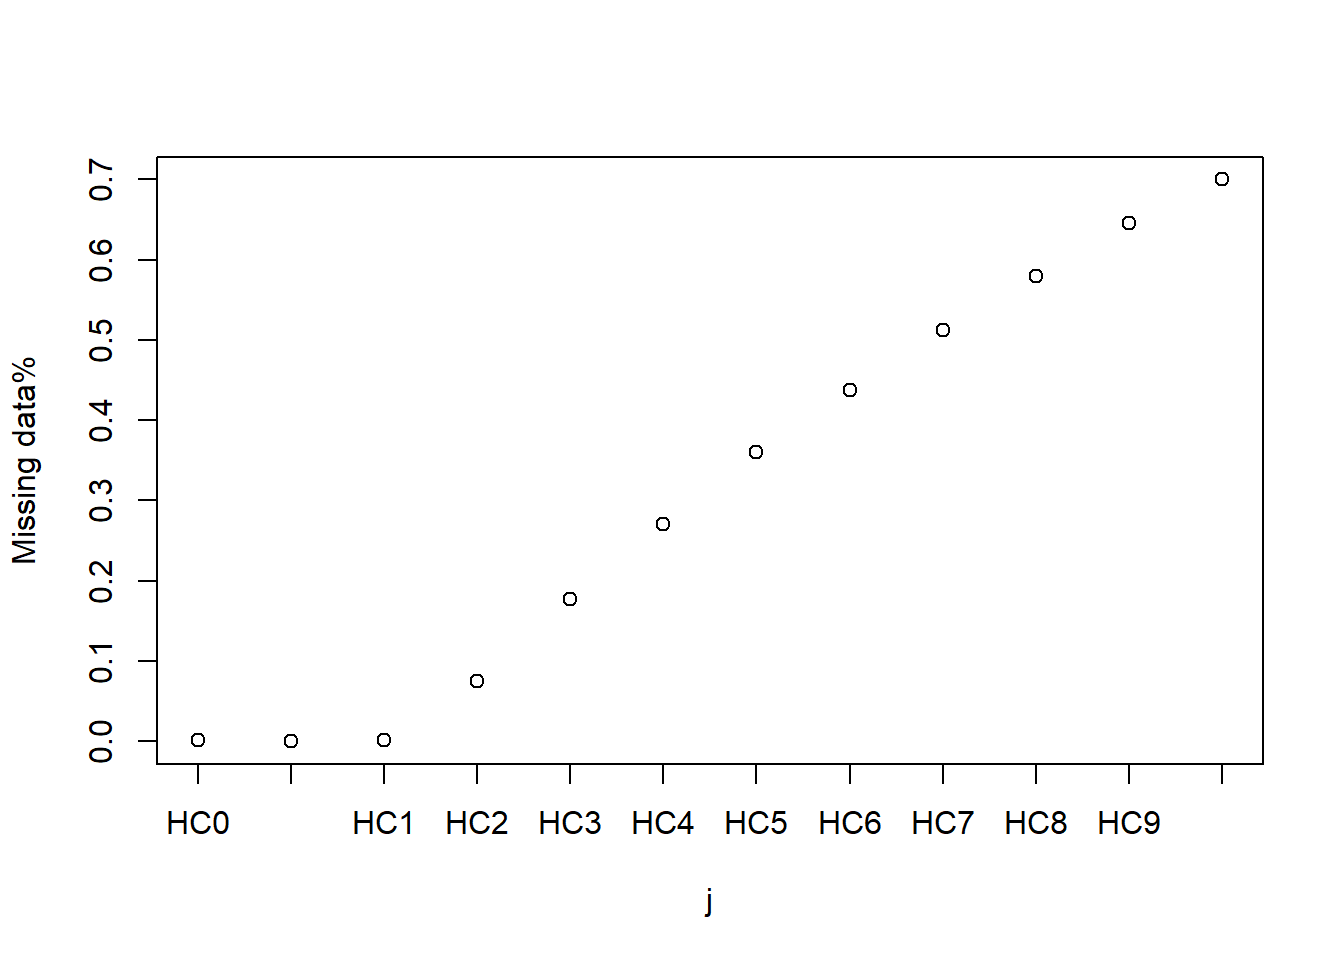
\includegraphics{Report_files/figure-latex/unnamed-chunk-3-1} \end{center}

Conclusion could be at the first three measurements, there are almost
full data More people tends to miss the measurements when time
increases. And then we can extract all NA data from the long table to
analyse their construction

\begin{Shaded}
\begin{Highlighting}[]
\NormalTok{trenal.long.NA }\OtherTok{=}\NormalTok{ trenal.long[}\FunctionTok{is.na}\NormalTok{(trenal.long}\SpecialCharTok{$}\NormalTok{Hc),]}
\CommentTok{\#t = unique(trenal.long.NA$id) \# 821 individuals}
\NormalTok{trenal.long.NA.unique }\OtherTok{\textless{}{-}}\NormalTok{ trenal.long.NA[}\FunctionTok{match}\NormalTok{( }\FunctionTok{unique}\NormalTok{(trenal.long.NA}\SpecialCharTok{$}\NormalTok{id), trenal.long.NA}\SpecialCharTok{$}\NormalTok{id),]}
\FunctionTok{summary}\NormalTok{(trenal.long.NA.unique)}
\end{Highlighting}
\end{Shaded}

\begin{verbatim}
##        id           age        male    cardio  reject        Hc     
##  1      :  1   Min.   :15.00   0:327   0:669   0:588   Min.   : NA  
##  2      :  1   1st Qu.:39.00   1:494   1:152   1:233   1st Qu.: NA  
##  4      :  1   Median :50.00                           Median : NA  
##  7      :  1   Mean   :48.31                           Mean   :NaN  
##  14     :  1   3rd Qu.:59.00                           3rd Qu.: NA  
##  18     :  1   Max.   :76.00                           Max.   : NA  
##  (Other):815   NA's   :1                               NA's   :821  
##       time       
##  Min.   : 0.000  
##  1st Qu.: 3.000  
##  Median : 5.000  
##  Mean   : 5.638  
##  3rd Qu.: 8.000  
##  Max.   :10.000  
## 
\end{verbatim}

\begin{Shaded}
\begin{Highlighting}[]
\DocumentationTok{\#\# Conclusion, For the missing data, we can see that }
\FunctionTok{png}\NormalTok{(}\AttributeTok{file=}\StringTok{"MissingValueAnalysis.png"}\NormalTok{,}
    \AttributeTok{width=}\DecValTok{600}\NormalTok{, }\AttributeTok{height=}\DecValTok{1200}\NormalTok{)}
\FunctionTok{plot.new}\NormalTok{()}
\FunctionTok{par}\NormalTok{(}\AttributeTok{mfrow=}\FunctionTok{c}\NormalTok{(}\DecValTok{4}\NormalTok{,}\DecValTok{2}\NormalTok{))}
\DocumentationTok{\#\# age }
\FunctionTok{hist}\NormalTok{(trenal.long.unique}\SpecialCharTok{$}\NormalTok{age,}\AttributeTok{title=}\StringTok{"Age distribution in original data"}\NormalTok{)}
\FunctionTok{hist}\NormalTok{(trenal.long.NA.unique}\SpecialCharTok{$}\NormalTok{age,}\AttributeTok{col=}\StringTok{"red"}\NormalTok{,}\AttributeTok{title=}\StringTok{"Age distribution in missing data"}\NormalTok{)}

\DocumentationTok{\#\# male}
\FunctionTok{plot}\NormalTok{(trenal.long.unique}\SpecialCharTok{$}\NormalTok{male)}
\FunctionTok{title}\NormalTok{(}\AttributeTok{main=}\StringTok{"Gender distribution in original data"}\NormalTok{)}
\FunctionTok{plot}\NormalTok{(trenal.long.NA.unique}\SpecialCharTok{$}\NormalTok{male,}\AttributeTok{col=}\StringTok{"red"}\NormalTok{)}
\FunctionTok{title}\NormalTok{(}\AttributeTok{main=}\StringTok{"Gender distribution in missing data"}\NormalTok{)}

\DocumentationTok{\#\# cardio}
\FunctionTok{plot}\NormalTok{(trenal.long.unique}\SpecialCharTok{$}\NormalTok{cardio)}
\FunctionTok{title}\NormalTok{(}\AttributeTok{main=}\StringTok{"Cardio distribution in original data"}\NormalTok{)}
\FunctionTok{plot}\NormalTok{(trenal.long.NA.unique}\SpecialCharTok{$}\NormalTok{cardio,}\AttributeTok{col=}\StringTok{"red"}\NormalTok{)}
\FunctionTok{title}\NormalTok{(}\AttributeTok{main=}\StringTok{"Cardio distribution in missing data"}\NormalTok{)}

\DocumentationTok{\#\# reject}
\FunctionTok{plot}\NormalTok{(trenal.long.unique}\SpecialCharTok{$}\NormalTok{reject)}
\FunctionTok{title}\NormalTok{(}\AttributeTok{main=}\StringTok{"Reject distribution in original data"}\NormalTok{)}
\FunctionTok{plot}\NormalTok{(trenal.long.NA.unique}\SpecialCharTok{$}\NormalTok{reject,}\AttributeTok{col=}\StringTok{"red"}\NormalTok{) }
\FunctionTok{title}\NormalTok{(}\AttributeTok{main=}\StringTok{"Reject distribution in missing data"}\NormalTok{)}
\FunctionTok{dev.off}\NormalTok{()}
\end{Highlighting}
\end{Shaded}

\begin{verbatim}
## pdf 
##   2
\end{verbatim}

The missing data has a similar distribution as the ideal full data set,
in age, male, cardio and reject plot. So we may conclude that the
missing data are random and not depend on any observed predictors or the
response. \# Exploratory Data Analysis

\hypertarget{univariate-summaries}{%
\subsection{Univariate summaries}\label{univariate-summaries}}

\hypertarget{plot-histogram-of-continuous-variables}{%
\subsubsection{Plot histogram of continuous
variables}\label{plot-histogram-of-continuous-variables}}

\begin{Shaded}
\begin{Highlighting}[]
\FunctionTok{hist}\NormalTok{(trenal.long}\SpecialCharTok{$}\NormalTok{Hc,}\AttributeTok{title=}\StringTok{"Hc distribution in original data"}\NormalTok{)}
\end{Highlighting}
\end{Shaded}

\begin{center}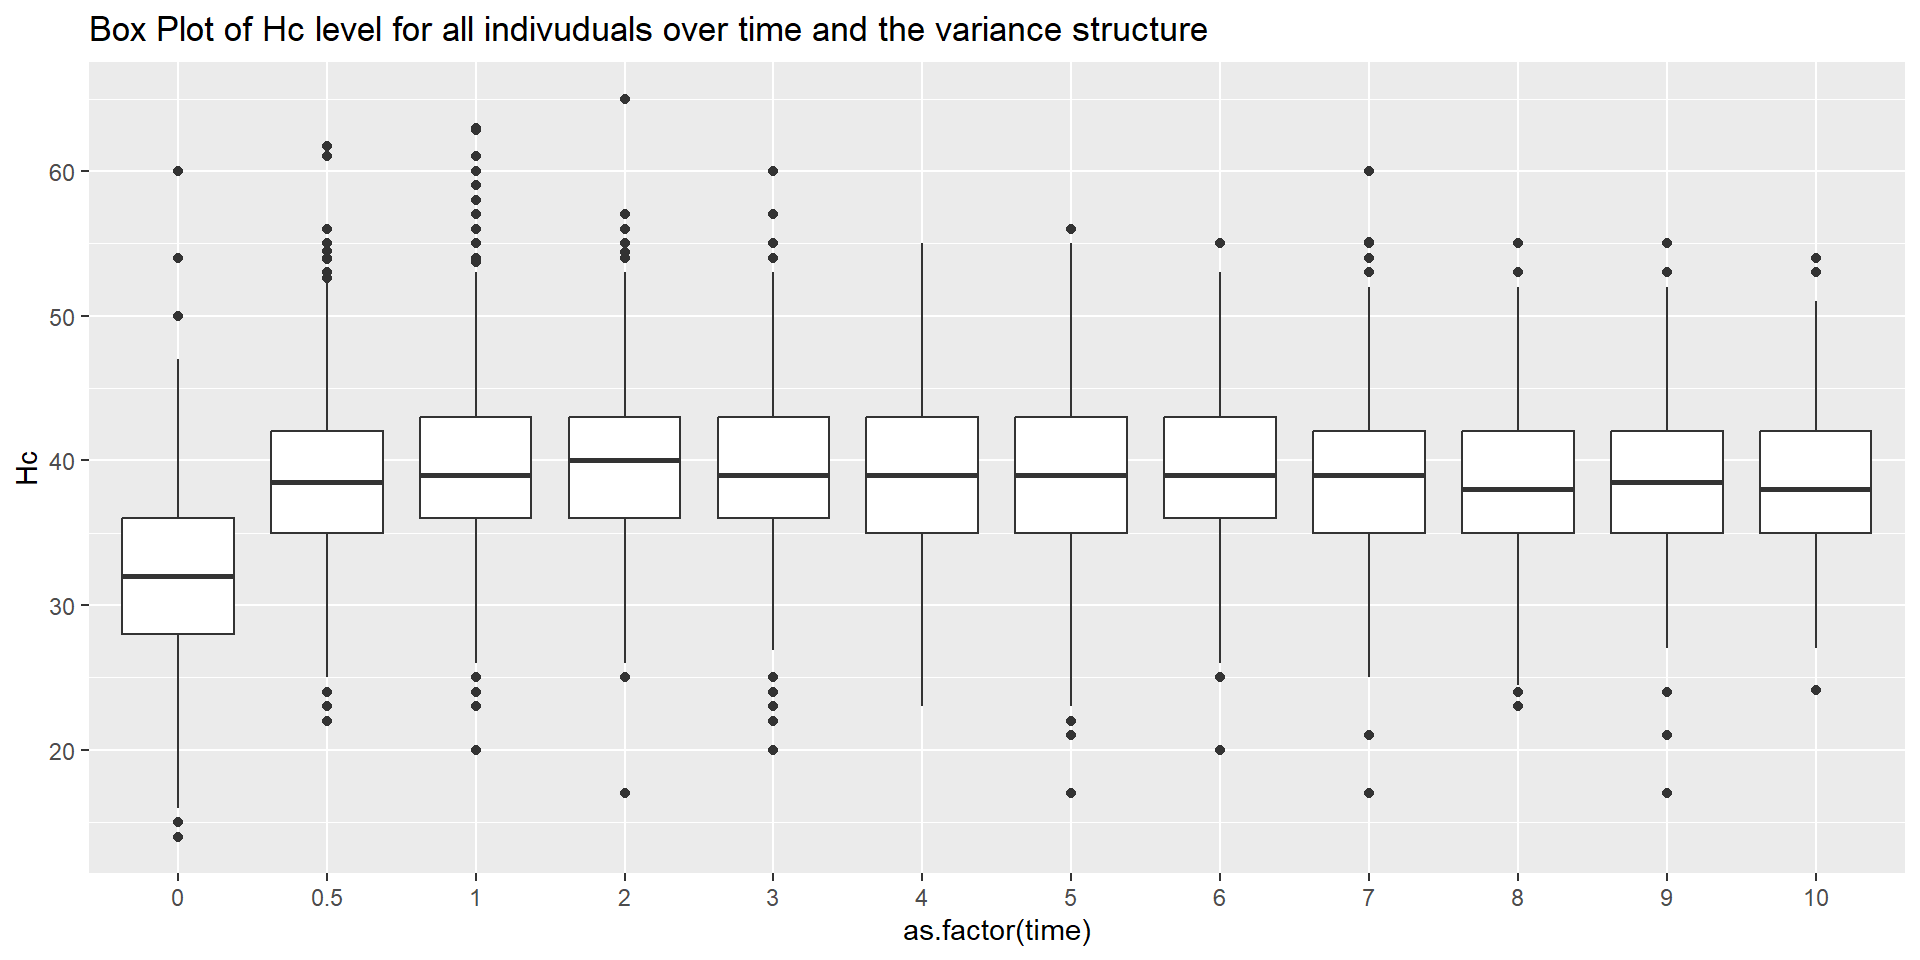
\includegraphics{Report_files/figure-latex/unnamed-chunk-6-1} \end{center}

\begin{Shaded}
\begin{Highlighting}[]
\FunctionTok{hist}\NormalTok{(trenal.long.unique}\SpecialCharTok{$}\NormalTok{age,}\AttributeTok{title=}\StringTok{"age distribution in original data"}\NormalTok{)}
\end{Highlighting}
\end{Shaded}

\begin{center}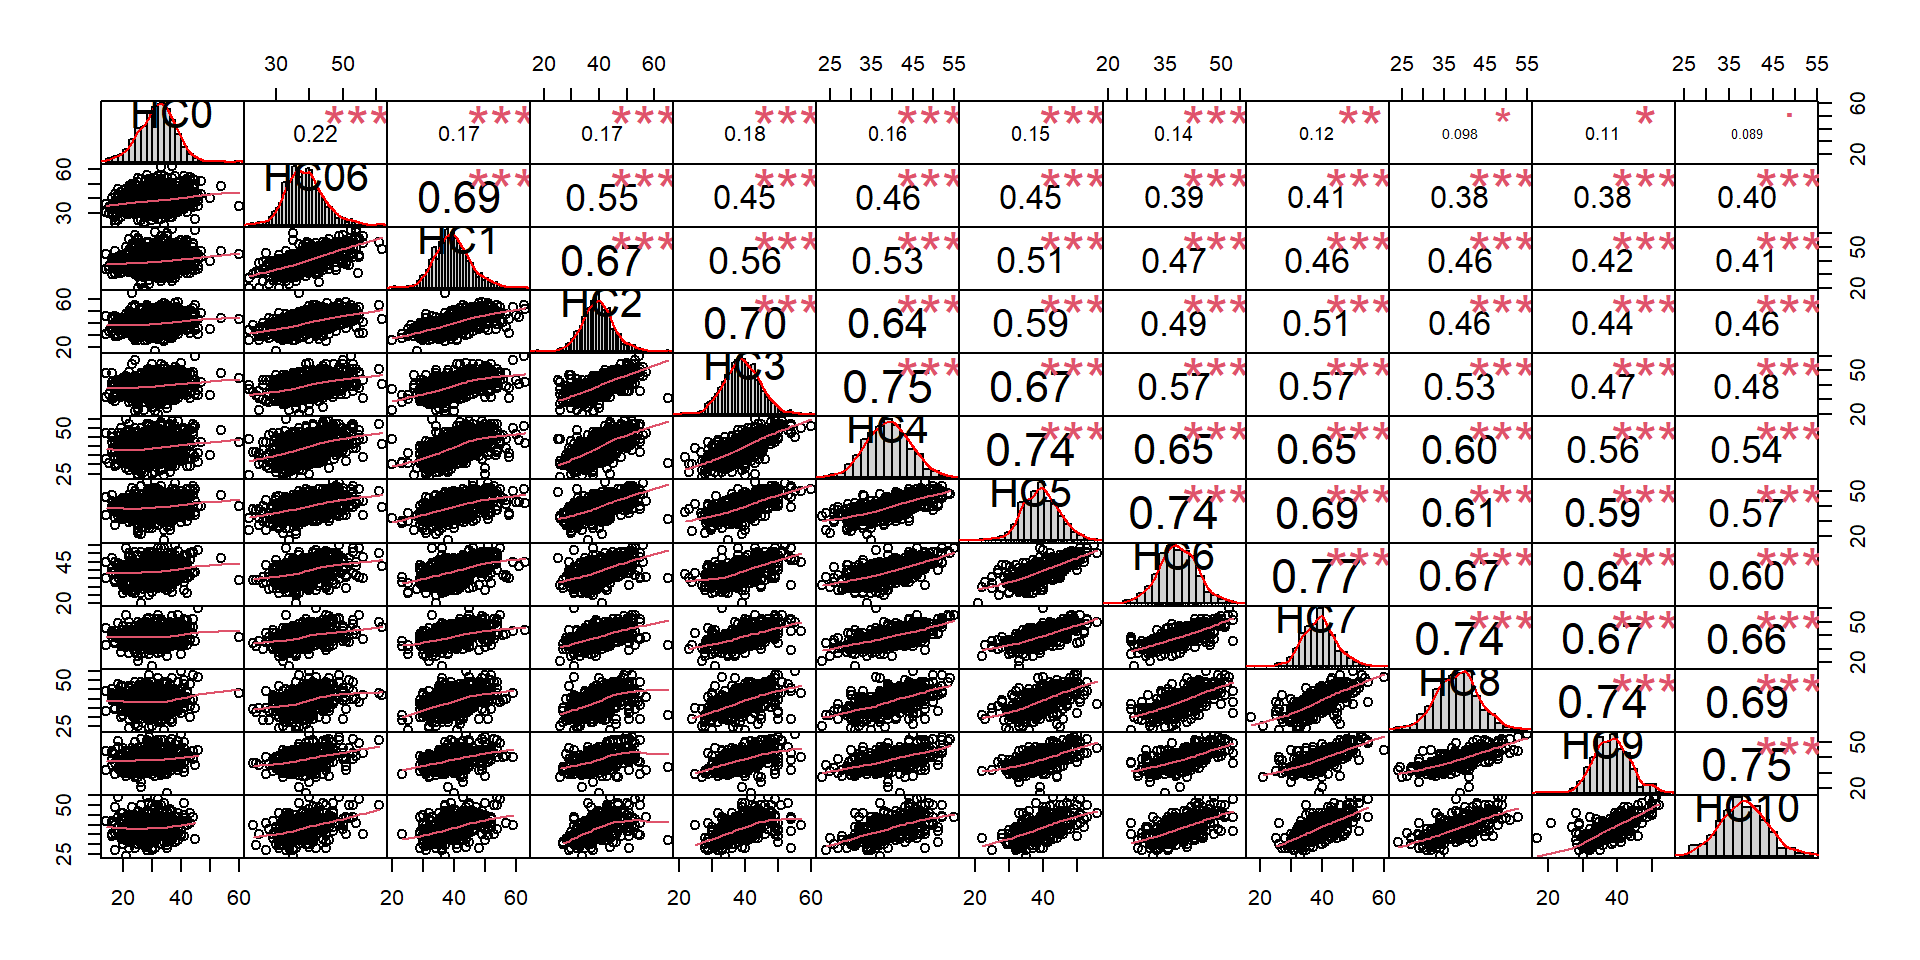
\includegraphics{Report_files/figure-latex/unnamed-chunk-7-1} \end{center}

\hypertarget{bivariate-summaries}{%
\subsection{Bivariate summaries}\label{bivariate-summaries}}

\hypertarget{plot-relationship-between-pairs-of-variables}{%
\subsubsection{Plot relationship between pairs of
variables}\label{plot-relationship-between-pairs-of-variables}}

\begin{Shaded}
\begin{Highlighting}[]
\CommentTok{\# Bivariate summaries}
\NormalTok{gg }\OtherTok{\textless{}{-}} \FunctionTok{ggpairs}\NormalTok{(}\AttributeTok{data=}\NormalTok{trenal.long.unique[,}\DecValTok{2}\SpecialCharTok{:}\DecValTok{6}\NormalTok{])}\CommentTok{\# Here Hc is only one value per individual}
\NormalTok{gg}
\end{Highlighting}
\end{Shaded}

\begin{center}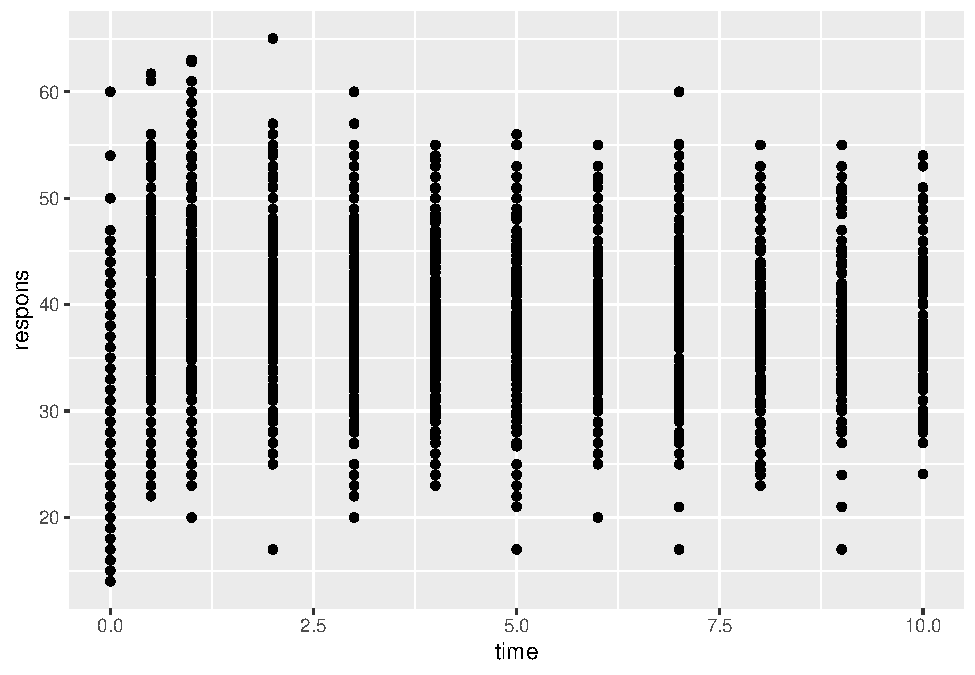
\includegraphics{Report_files/figure-latex/unnamed-chunk-8-1} \end{center}

\hypertarget{plot-the-time-trend-of-response}{%
\subsubsection{Plot the time trend of
response}\label{plot-the-time-trend-of-response}}

\hypertarget{mean-structure}{%
\paragraph{Mean Structure}\label{mean-structure}}

\begin{Shaded}
\begin{Highlighting}[]
\CommentTok{\# To view the mean structure of the Hc for all individuals}
\FunctionTok{ggplot}\NormalTok{(trenal.long.noNA,}\FunctionTok{aes}\NormalTok{(}\AttributeTok{x=}\FunctionTok{as.factor}\NormalTok{(time),}\AttributeTok{y=}\NormalTok{Hc,}\AttributeTok{group=}\NormalTok{id))  }\SpecialCharTok{+} \FunctionTok{geom\_line}\NormalTok{(}\AttributeTok{col=}\StringTok{"grey"}\NormalTok{)}\SpecialCharTok{+}\FunctionTok{stat\_summary}\NormalTok{(}\FunctionTok{aes}\NormalTok{(}\AttributeTok{group=}\DecValTok{1}\NormalTok{),}\AttributeTok{geom=}\StringTok{"line"}\NormalTok{,}\AttributeTok{fun=}\NormalTok{mean,}\AttributeTok{linewidth=}\DecValTok{2}\NormalTok{)}\SpecialCharTok{+}
  \FunctionTok{labs}\NormalTok{(}\AttributeTok{title=}\StringTok{"Line plot of Hc level for all individuals overtime and the mean structure"}\NormalTok{)}
\end{Highlighting}
\end{Shaded}

\begin{center}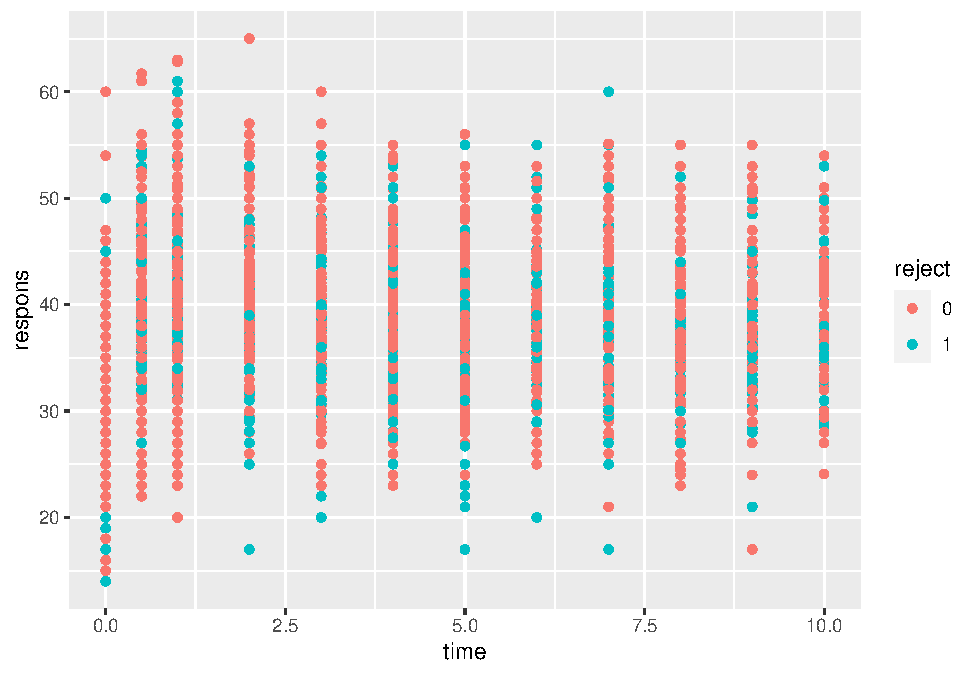
\includegraphics{Report_files/figure-latex/unnamed-chunk-9-1} \end{center}

\hypertarget{variance-structure}{%
\paragraph{Variance Structure}\label{variance-structure}}

\begin{Shaded}
\begin{Highlighting}[]
\CommentTok{\# To view to variance structure}
\FunctionTok{ggplot}\NormalTok{(trenal.long.noNA,}\FunctionTok{aes}\NormalTok{(}\AttributeTok{x=}\FunctionTok{as.factor}\NormalTok{(time),}\AttributeTok{y=}\NormalTok{Hc))}\SpecialCharTok{+} 
  \FunctionTok{geom\_boxplot}\NormalTok{(}\AttributeTok{position=}\FunctionTok{position\_dodge}\NormalTok{(}\DecValTok{1}\NormalTok{))}\SpecialCharTok{+}
  \FunctionTok{labs}\NormalTok{(}\AttributeTok{title=}\StringTok{"Box Plot of Hc level for all indivuduals over time and the variance structure"}\NormalTok{)}
\end{Highlighting}
\end{Shaded}

\begin{center}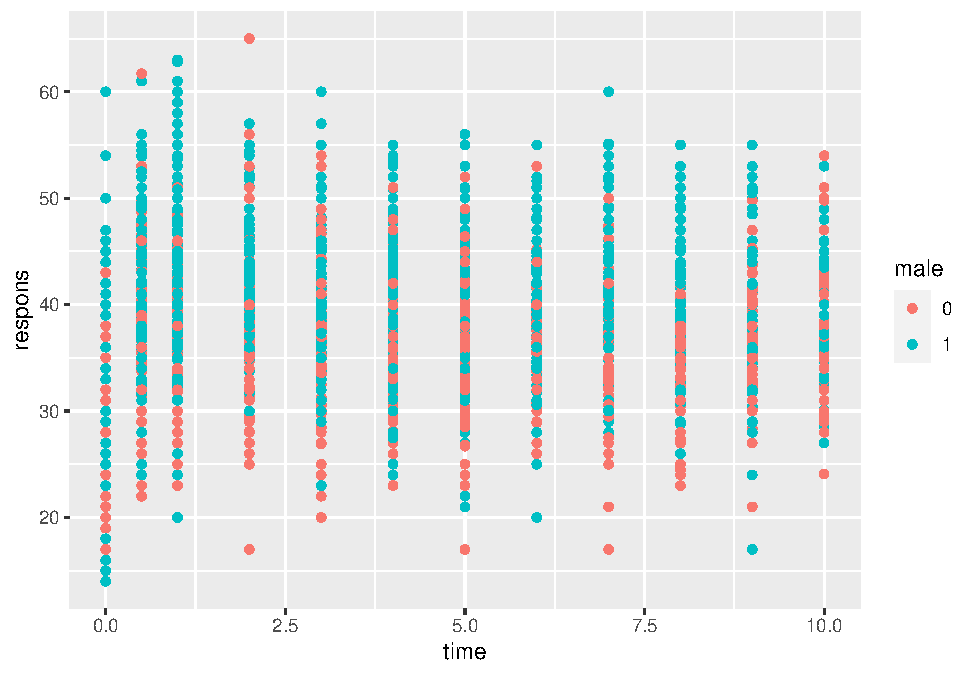
\includegraphics{Report_files/figure-latex/unnamed-chunk-10-1} \end{center}

\hypertarget{covariance-structure}{%
\paragraph{Covariance Structure}\label{covariance-structure}}

\begin{Shaded}
\begin{Highlighting}[]
\NormalTok{HcCorr }\OtherTok{=}\NormalTok{ trenal.wide[,}\FunctionTok{c}\NormalTok{(}\DecValTok{1}\SpecialCharTok{:}\DecValTok{12}\NormalTok{)]}
\CommentTok{\#cor(HcCorr,use="complete.obs" ) \# also COV for covariance}
\FunctionTok{chart.Correlation}\NormalTok{(HcCorr,}\AttributeTok{historgram=}\ConstantTok{TRUE}\NormalTok{)}
\end{Highlighting}
\end{Shaded}

\begin{center}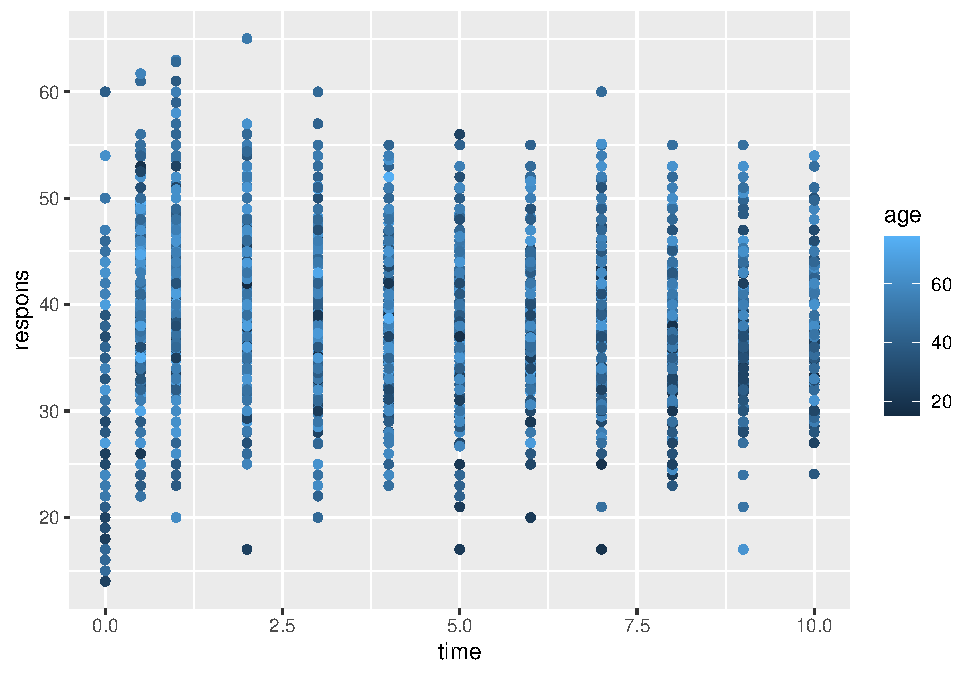
\includegraphics{Report_files/figure-latex/unnamed-chunk-11-1} \end{center}

\hypertarget{find-out-a-covariate-increasing-or-decreasing-the-responses-time-trend}{%
\subsubsection{Find out a covariate increasing or decreasing the
responses time
trend}\label{find-out-a-covariate-increasing-or-decreasing-the-responses-time-trend}}

\hypertarget{spaghetti-plot}{%
\paragraph{Spaghetti Plot}\label{spaghetti-plot}}

\begin{Shaded}
\begin{Highlighting}[]
\CommentTok{\# since the data dimension is large 9551 x 8, we can select random 30 data to have a look }
\FunctionTok{set.seed}\NormalTok{(}\DecValTok{1}\NormalTok{)}
\NormalTok{selected }\OtherTok{\textless{}{-}} \FunctionTok{sample}\NormalTok{(}\DecValTok{1}\SpecialCharTok{:}\FunctionTok{length}\NormalTok{(}\FunctionTok{unique}\NormalTok{(trenal.long.noNA}\SpecialCharTok{$}\NormalTok{id)),}\DecValTok{30}\NormalTok{,}\AttributeTok{replace=}\NormalTok{T) }\CommentTok{\# random samples and permutations}
\CommentTok{\#selected.vector = as.vector(selected)}
\NormalTok{data.selected }\OtherTok{=}\NormalTok{ trenal.long.noNA[(trenal.long.noNA}\SpecialCharTok{$}\NormalTok{id }\SpecialCharTok{\%in\%} \FunctionTok{c}\NormalTok{(selected)), ] }
\end{Highlighting}
\end{Shaded}

\begin{itemize}
\tightlist
\item
  Spaghetti plot group by id
\end{itemize}

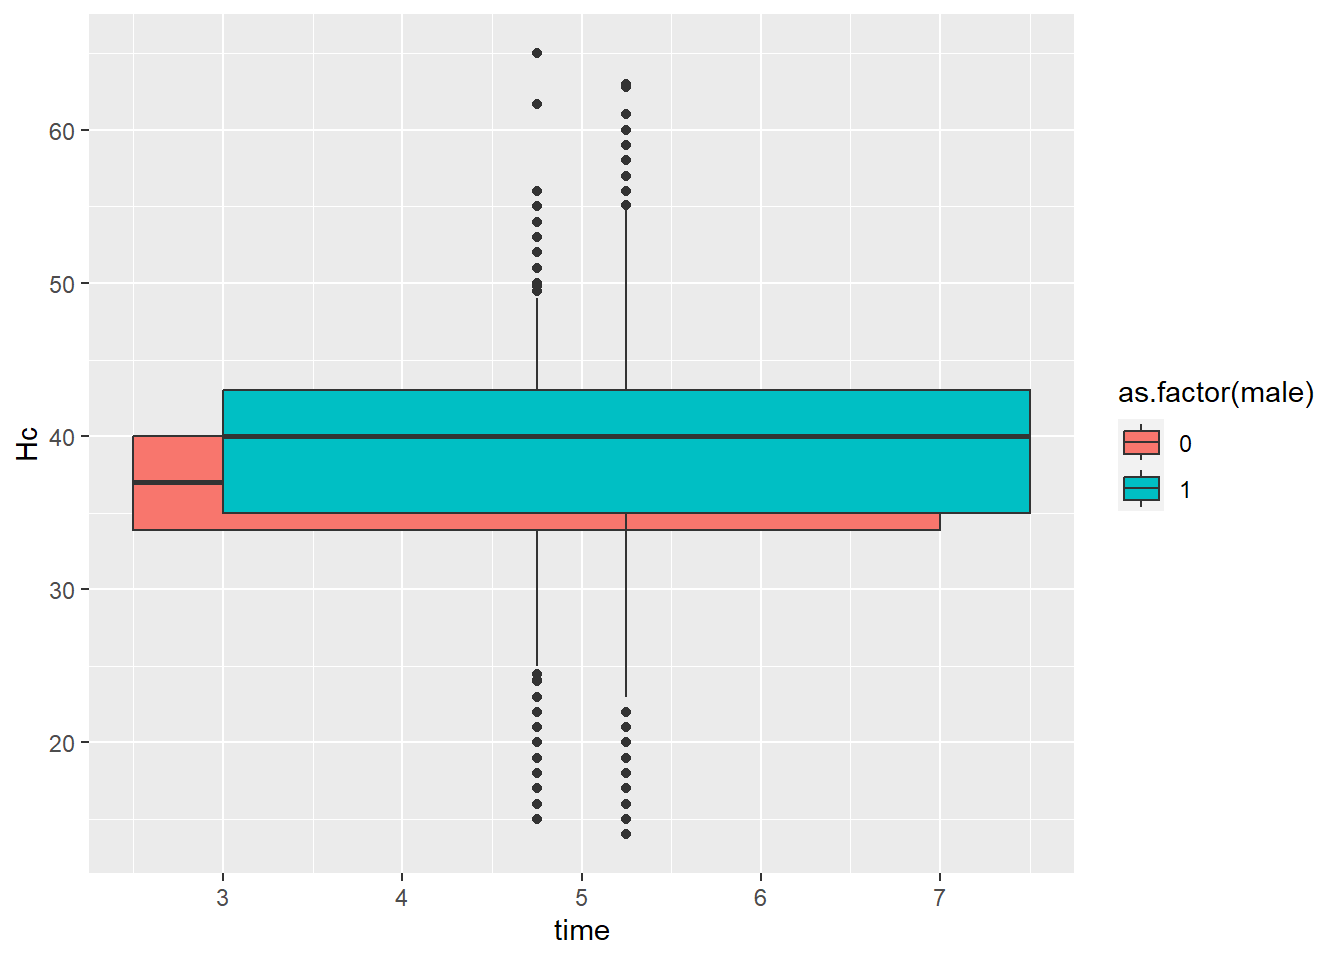
\includegraphics{Report_files/figure-latex/unnamed-chunk-13-1.pdf}

\begin{itemize}
\tightlist
\item
  Spaghetti plot group by male
\end{itemize}

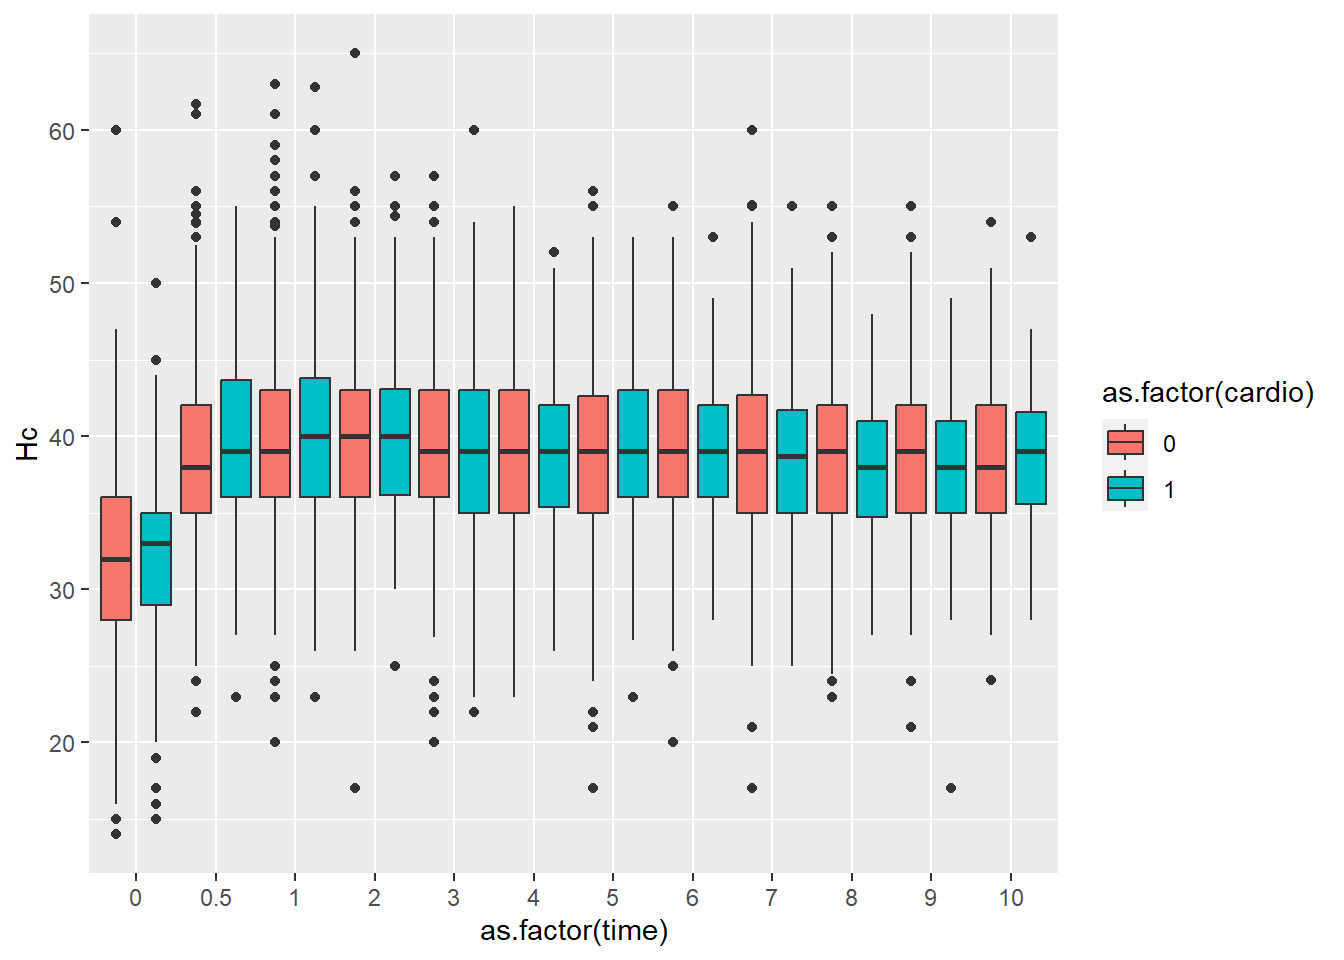
\includegraphics{Report_files/figure-latex/unnamed-chunk-14-1.pdf}

\begin{itemize}
\tightlist
\item
  Spaghetti plot group by cardio
\end{itemize}

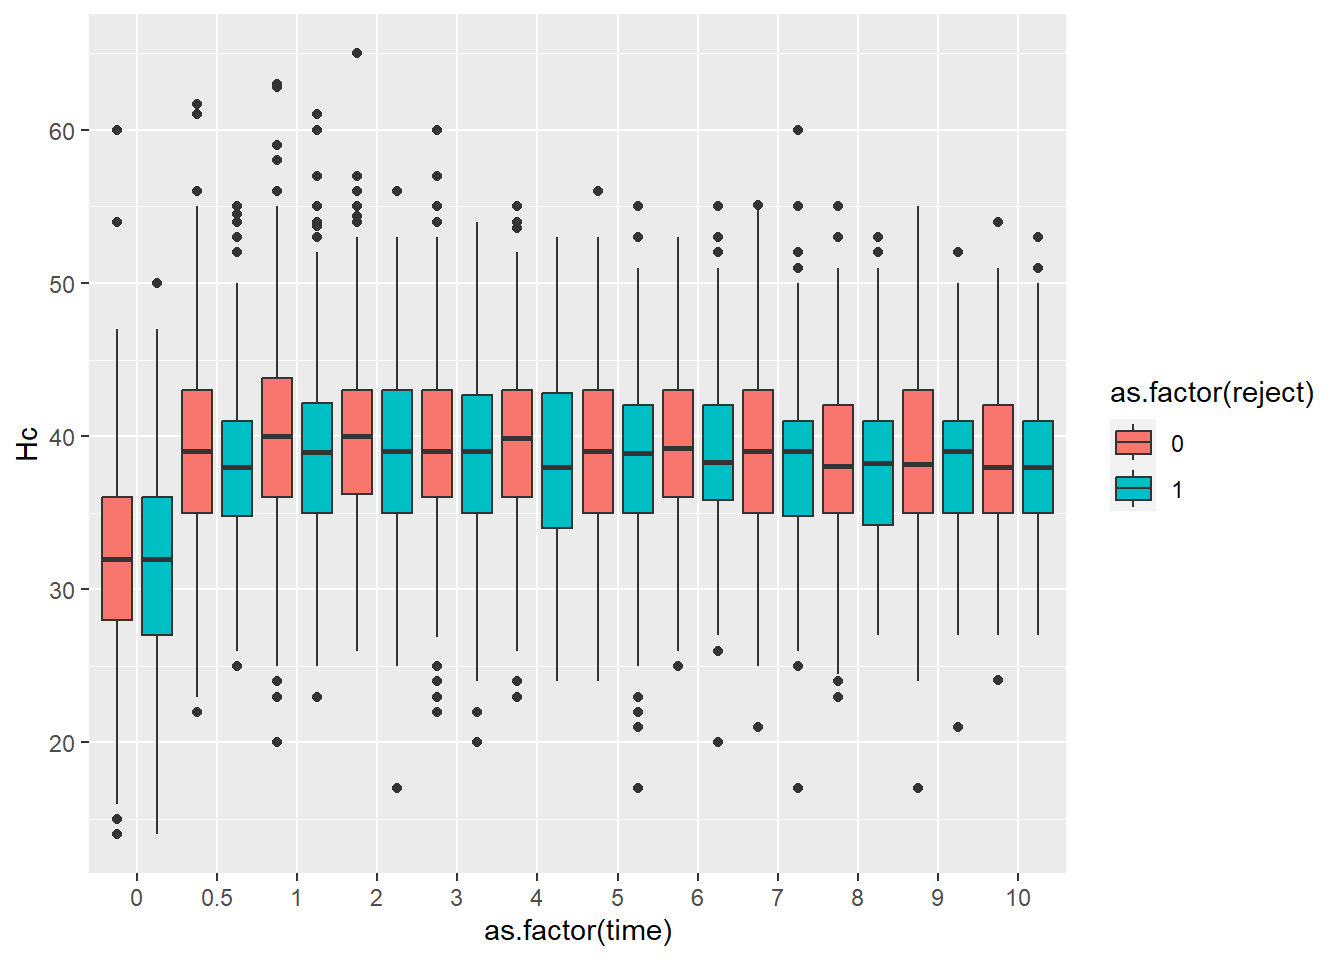
\includegraphics{Report_files/figure-latex/unnamed-chunk-15-1.pdf}

*Spaghetti plot group by reject

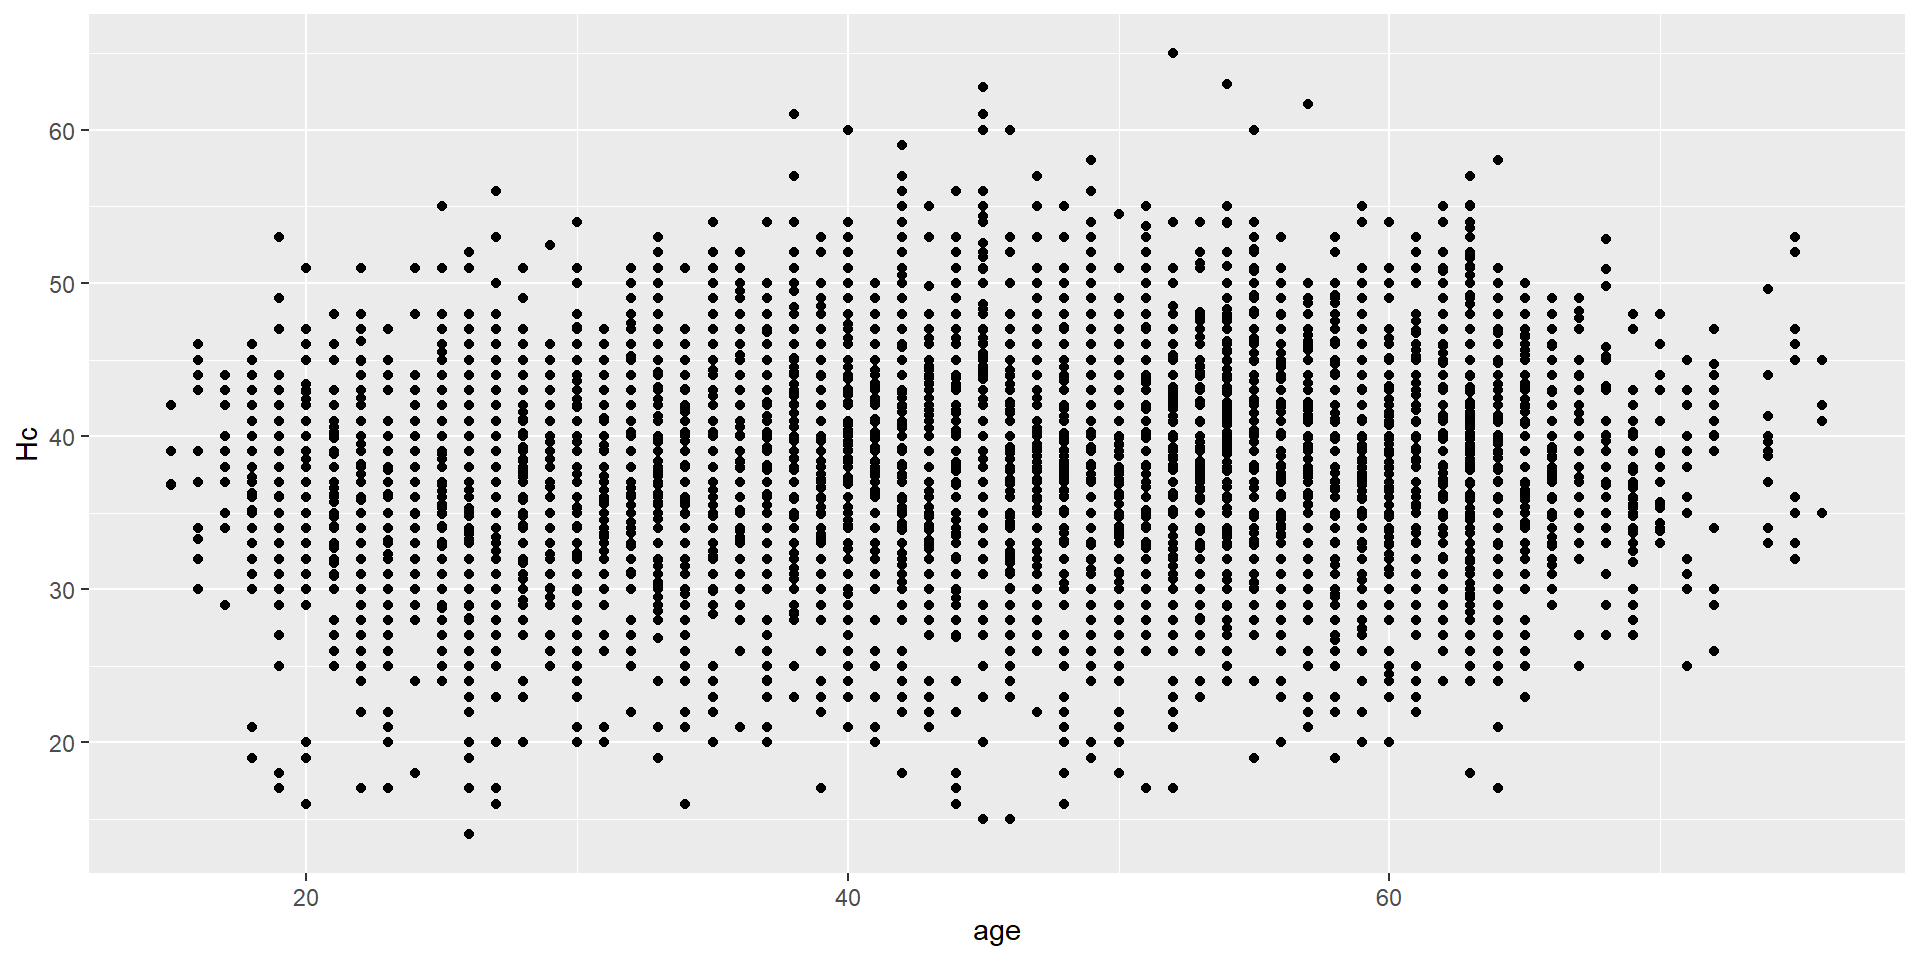
\includegraphics{Report_files/figure-latex/unnamed-chunk-16-1.pdf}

\hypertarget{boxplot}{%
\paragraph{Boxplot}\label{boxplot}}

\begin{itemize}
\tightlist
\item
  Box plot by male
\end{itemize}

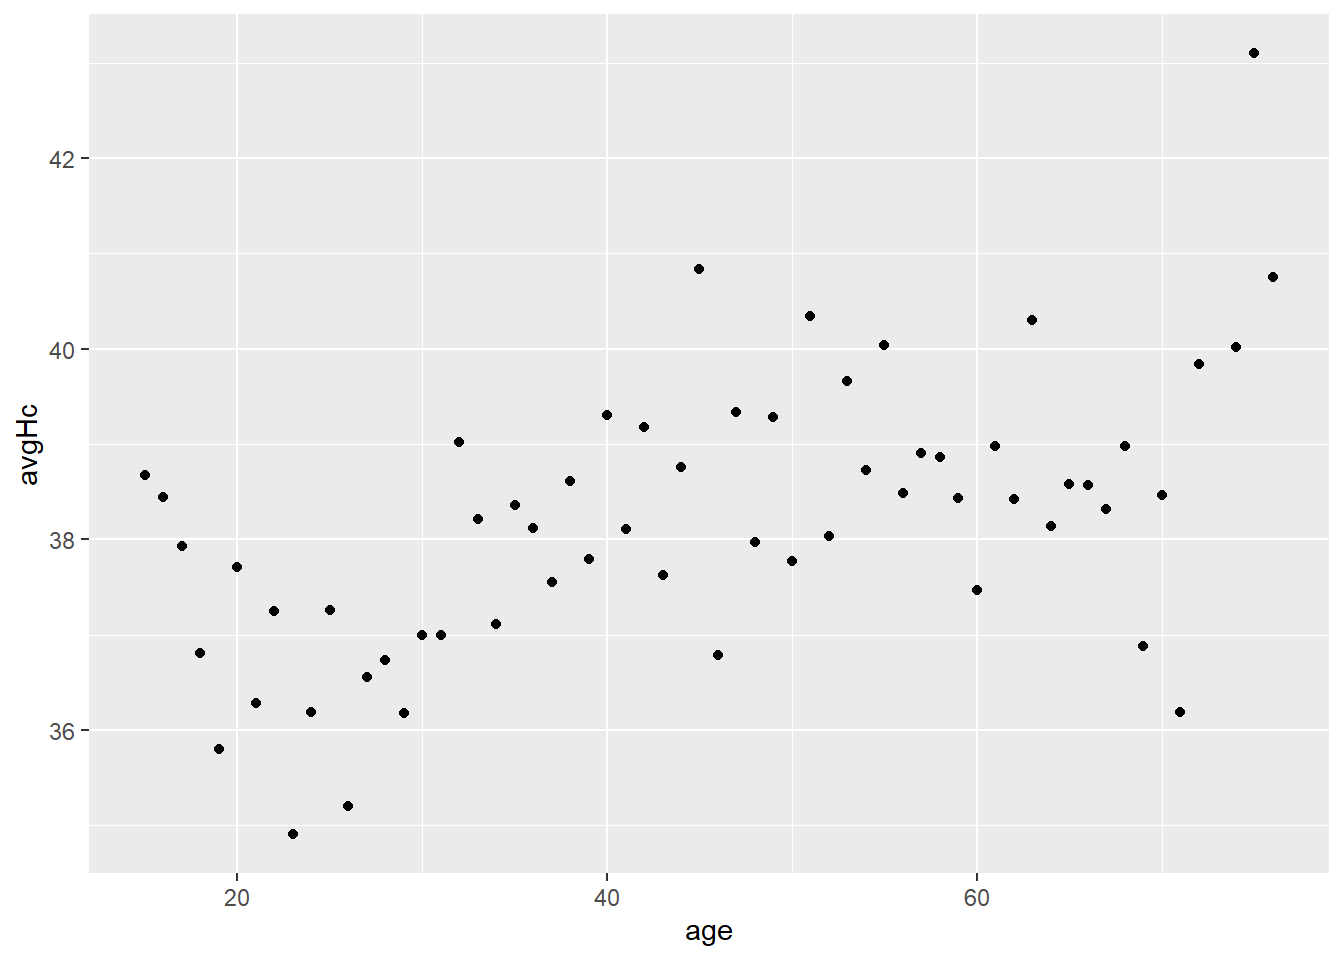
\includegraphics{Report_files/figure-latex/unnamed-chunk-17-1.pdf}

\begin{itemize}
\tightlist
\item
  Box plot by cardio
\end{itemize}

\begin{center}\includegraphics{Report_files/figure-latex/unnamed-chunk-18-1} \end{center}

\begin{itemize}
\tightlist
\item
  Box plot by reject
\end{itemize}

\includegraphics{Report_files/figure-latex/unnamed-chunk-19-1.pdf}

\hypertarget{data-set-analysis-to-see-the-age-effect}{%
\subsubsection{Data set analysis to see the age
effect}\label{data-set-analysis-to-see-the-age-effect}}

\begin{Shaded}
\begin{Highlighting}[]
\FunctionTok{ggplot}\NormalTok{(}\AttributeTok{data=}\NormalTok{trenal.long.noNA,}\FunctionTok{aes}\NormalTok{(}\AttributeTok{y=}\NormalTok{Hc,}\AttributeTok{x=}\NormalTok{age))}\SpecialCharTok{+}\FunctionTok{geom\_point}\NormalTok{()}
\end{Highlighting}
\end{Shaded}

\includegraphics{Report_files/figure-latex/unnamed-chunk-20-1.pdf}

\begin{Shaded}
\begin{Highlighting}[]
\NormalTok{data.groupbyage }\OtherTok{\textless{}{-}}\NormalTok{ trenal.long.noNA }\SpecialCharTok{\%\textgreater{}\%}   \FunctionTok{group\_by}\NormalTok{(age) }\SpecialCharTok{\%\textgreater{}\%} \FunctionTok{summarise}\NormalTok{(}\AttributeTok{avgHc=}\FunctionTok{mean}\NormalTok{(Hc))}
\FunctionTok{ggplot}\NormalTok{(}\AttributeTok{data=}\NormalTok{data.groupbyage,}\FunctionTok{aes}\NormalTok{(}\AttributeTok{y=}\NormalTok{avgHc,}\AttributeTok{x=}\NormalTok{age))}\SpecialCharTok{+}\FunctionTok{geom\_point}\NormalTok{()}
\end{Highlighting}
\end{Shaded}

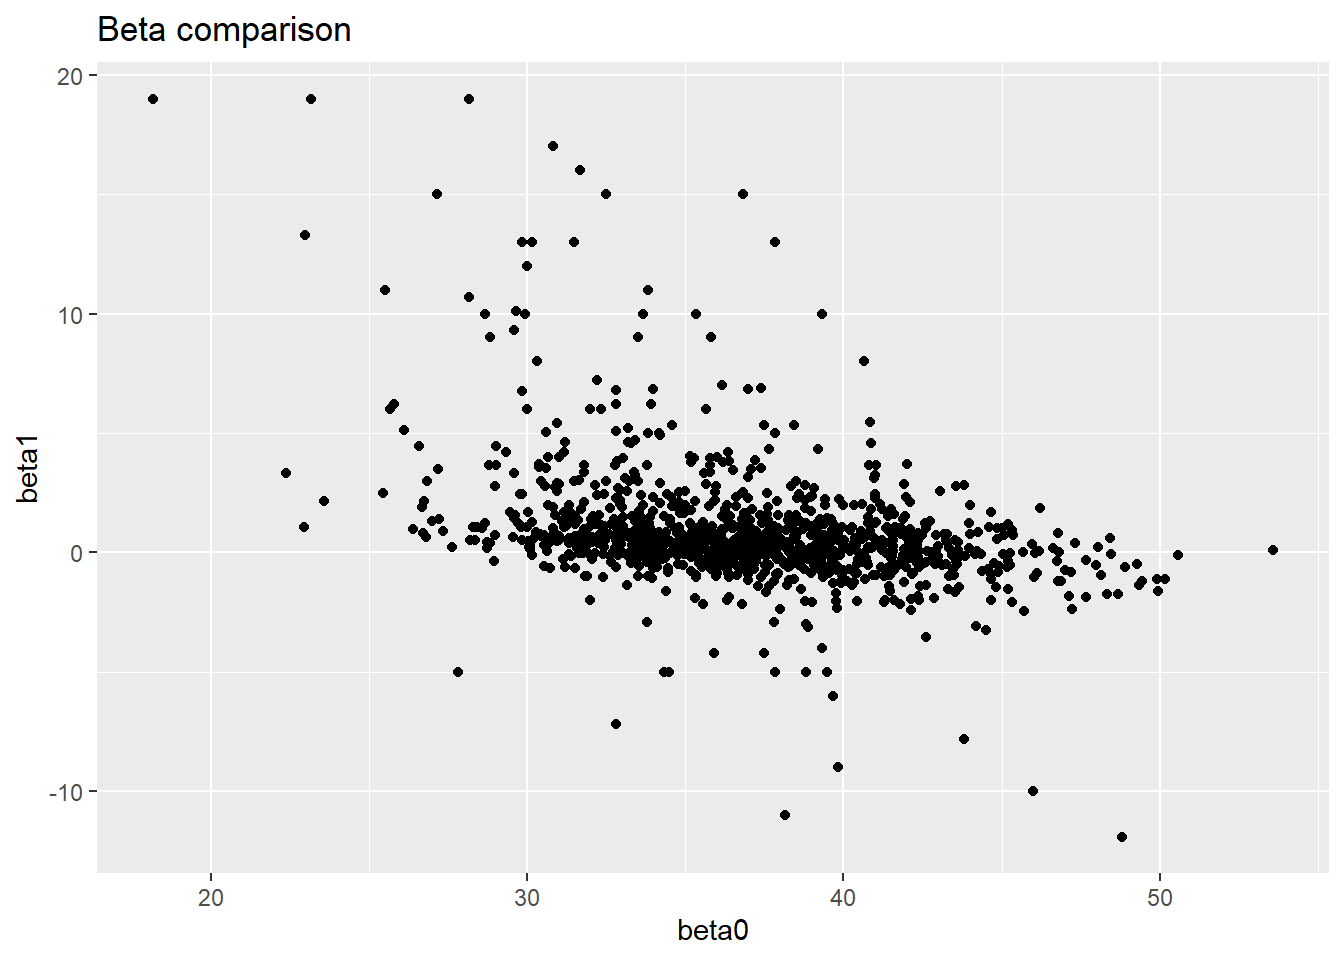
\includegraphics{Report_files/figure-latex/unnamed-chunk-21-1.pdf}

\hypertarget{conclusions-after-exploring-data-analysis}{%
\subsection{Conclusions after exploring data
analysis}\label{conclusions-after-exploring-data-analysis}}

\begin{itemize}
\tightlist
\item
  The Hc time trend tends to increase first from 0 to 0.5 year then keep
  variated during the rest of the meassurements
\item
  The subject related variables age may increase the mean Hc level of a
  subject
\item
  Male has relative higher Hc level than female
\item
  Cardio or reject play no big difference in the Hc level measurements.
\end{itemize}

\hypertarget{multilevel-data-analysis}{%
\section{Multilevel Data Analysis}\label{multilevel-data-analysis}}

\hypertarget{multivariate-linear-model-analysis}{%
\subsection{Multivariate Linear Model
Analysis}\label{multivariate-linear-model-analysis}}

\begin{Shaded}
\begin{Highlighting}[]
\NormalTok{lm1 }\OtherTok{\textless{}{-}} \FunctionTok{lm}\NormalTok{(Hc }\SpecialCharTok{\textasciitilde{}}\NormalTok{ time, trenal.long)}
\FunctionTok{summary}\NormalTok{(lm1)}
\end{Highlighting}
\end{Shaded}

\begin{verbatim}
## 
## Call:
## lm(formula = Hc ~ time, data = trenal.long)
## 
## Residuals:
##      Min       1Q   Median       3Q      Max 
## -23.3368  -3.8633   0.0393   3.8206  27.1367 
## 
## Coefficients:
##             Estimate Std. Error t value Pr(>|t|)    
## (Intercept) 37.33685    0.09410   396.8   <2e-16 ***
## time         0.26322    0.02073    12.7   <2e-16 ***
## ---
## Signif. codes:  0 '***' 0.001 '**' 0.01 '*' 0.05 '.' 0.1 ' ' 1
## 
## Residual standard error: 6.023 on 9556 degrees of freedom
##   (4362 observations deleted due to missingness)
## Multiple R-squared:  0.01659,    Adjusted R-squared:  0.01648 
## F-statistic: 161.2 on 1 and 9556 DF,  p-value: < 2.2e-16
\end{verbatim}

\begin{Shaded}
\begin{Highlighting}[]
\NormalTok{lm2 }\OtherTok{\textless{}{-}} \FunctionTok{lm}\NormalTok{(Hc }\SpecialCharTok{\textasciitilde{}}\NormalTok{ time }\SpecialCharTok{+}\NormalTok{ age, trenal.long)}
\FunctionTok{summary}\NormalTok{(lm2)}
\end{Highlighting}
\end{Shaded}

\begin{verbatim}
## 
## Call:
## lm(formula = Hc ~ time + age, data = trenal.long)
## 
## Residuals:
##      Min       1Q   Median       3Q      Max 
## -24.0281  -3.7975  -0.0066   3.8187  26.7575 
## 
## Coefficients:
##              Estimate Std. Error t value Pr(>|t|)    
## (Intercept) 34.412259   0.238262  144.43   <2e-16 ***
## time         0.290850   0.020655   14.08   <2e-16 ***
## age          0.062472   0.004685   13.33   <2e-16 ***
## ---
## Signif. codes:  0 '***' 0.001 '**' 0.01 '*' 0.05 '.' 0.1 ' ' 1
## 
## Residual standard error: 5.969 on 9548 degrees of freedom
##   (4369 observations deleted due to missingness)
## Multiple R-squared:  0.03456,    Adjusted R-squared:  0.03436 
## F-statistic: 170.9 on 2 and 9548 DF,  p-value: < 2.2e-16
\end{verbatim}

\begin{Shaded}
\begin{Highlighting}[]
\NormalTok{lm3 }\OtherTok{\textless{}{-}} \FunctionTok{lm}\NormalTok{(Hc }\SpecialCharTok{\textasciitilde{}}\NormalTok{ time }\SpecialCharTok{+}\NormalTok{ age }\SpecialCharTok{+}\NormalTok{ male,trenal.long)}
\FunctionTok{summary}\NormalTok{(lm3)}
\end{Highlighting}
\end{Shaded}

\begin{verbatim}
## 
## Call:
## lm(formula = Hc ~ time + age + male, data = trenal.long)
## 
## Residuals:
##      Min       1Q   Median       3Q      Max 
## -25.1890  -3.7042   0.1498   3.6798  28.1470 
## 
## Coefficients:
##              Estimate Std. Error t value Pr(>|t|)    
## (Intercept) 32.981301   0.243570  135.41   <2e-16 ***
## time         0.303662   0.020230   15.01   <2e-16 ***
## age          0.062775   0.004586   13.69   <2e-16 ***
## male1        2.457069   0.120470   20.40   <2e-16 ***
## ---
## Signif. codes:  0 '***' 0.001 '**' 0.01 '*' 0.05 '.' 0.1 ' ' 1
## 
## Residual standard error: 5.843 on 9547 degrees of freedom
##   (4369 observations deleted due to missingness)
## Multiple R-squared:  0.07487,    Adjusted R-squared:  0.07458 
## F-statistic: 257.5 on 3 and 9547 DF,  p-value: < 2.2e-16
\end{verbatim}

\begin{Shaded}
\begin{Highlighting}[]
\NormalTok{lm4 }\OtherTok{\textless{}{-}} \FunctionTok{lm}\NormalTok{(Hc }\SpecialCharTok{\textasciitilde{}}\NormalTok{ time }\SpecialCharTok{+}\NormalTok{ age }\SpecialCharTok{+}\NormalTok{ male }\SpecialCharTok{+}\NormalTok{ reject,trenal.long)}
\FunctionTok{summary}\NormalTok{(lm4)}
\end{Highlighting}
\end{Shaded}

\begin{verbatim}
## 
## Call:
## lm(formula = Hc ~ time + age + male + reject, data = trenal.long)
## 
## Residuals:
##      Min       1Q   Median       3Q      Max 
## -25.2661  -3.6913   0.1555   3.7073  28.0424 
## 
## Coefficients:
##              Estimate Std. Error t value Pr(>|t|)    
## (Intercept) 33.194768   0.256818 129.254  < 2e-16 ***
## time         0.305407   0.020235  15.093  < 2e-16 ***
## age          0.060616   0.004659  13.011  < 2e-16 ***
## male1        2.443227   0.120550  20.267  < 2e-16 ***
## reject1     -0.336228   0.128591  -2.615  0.00894 ** 
## ---
## Signif. codes:  0 '***' 0.001 '**' 0.01 '*' 0.05 '.' 0.1 ' ' 1
## 
## Residual standard error: 5.841 on 9546 degrees of freedom
##   (4369 observations deleted due to missingness)
## Multiple R-squared:  0.07553,    Adjusted R-squared:  0.07514 
## F-statistic:   195 on 4 and 9546 DF,  p-value: < 2.2e-16
\end{verbatim}

\begin{Shaded}
\begin{Highlighting}[]
\NormalTok{lm5 }\OtherTok{\textless{}{-}} \FunctionTok{lm}\NormalTok{(Hc }\SpecialCharTok{\textasciitilde{}}\NormalTok{ time }\SpecialCharTok{+}\NormalTok{ age }\SpecialCharTok{+}\NormalTok{ male }\SpecialCharTok{+}\NormalTok{ reject }\SpecialCharTok{+}\NormalTok{ cardio,trenal.long)}
\FunctionTok{summary}\NormalTok{(lm5)}
\end{Highlighting}
\end{Shaded}

\begin{verbatim}
## 
## Call:
## lm(formula = Hc ~ time + age + male + reject + cardio, data = trenal.long)
## 
## Residuals:
##      Min       1Q   Median       3Q      Max 
## -24.9829  -3.6915   0.1453   3.6927  27.9570 
## 
## Coefficients:
##              Estimate Std. Error t value Pr(>|t|)    
## (Intercept) 33.103534   0.259284 127.673   <2e-16 ***
## time         0.305654   0.020229  15.109   <2e-16 ***
## age          0.064002   0.004847  13.204   <2e-16 ***
## male1        2.449916   0.120545  20.324   <2e-16 ***
## reject1     -0.323401   0.128656  -2.514   0.0120 *  
## cardio1     -0.417558   0.165619  -2.521   0.0117 *  
## ---
## Signif. codes:  0 '***' 0.001 '**' 0.01 '*' 0.05 '.' 0.1 ' ' 1
## 
## Residual standard error: 5.84 on 9545 degrees of freedom
##   (4369 observations deleted due to missingness)
## Multiple R-squared:  0.07615,    Adjusted R-squared:  0.07566 
## F-statistic: 157.3 on 5 and 9545 DF,  p-value: < 2.2e-16
\end{verbatim}

\begin{Shaded}
\begin{Highlighting}[]
\FunctionTok{anova}\NormalTok{(lm2,lm3,lm4,lm5)}
\end{Highlighting}
\end{Shaded}

\begin{verbatim}
## Analysis of Variance Table
## 
## Model 1: Hc ~ time + age
## Model 2: Hc ~ time + age + male
## Model 3: Hc ~ time + age + male + reject
## Model 4: Hc ~ time + age + male + reject + cardio
##   Res.Df    RSS Df Sum of Sq        F    Pr(>F)    
## 1   9548 340135                                    
## 2   9547 325933  1   14201.6 416.4704 < 2.2e-16 ***
## 3   9546 325700  1     233.3   6.8405  0.008925 ** 
## 4   9545 325483  1     216.8   6.3564  0.011712 *  
## ---
## Signif. codes:  0 '***' 0.001 '**' 0.01 '*' 0.05 '.' 0.1 ' ' 1
\end{verbatim}

Conclustions: Variables must keep are: intercept, time, age, male if p
value is 0.01, it is better to add reject if p value is 0.05, it is
better to add cardio

\hypertarget{linear-mixed-effects-model-analysis}{%
\subsection{Linear Mixed effects Model
Analysis}\label{linear-mixed-effects-model-analysis}}

This is inspired from the chapter of
\url{https://bookdown.org/roback/bookdown-BeyondMLR/ch-lon.html}
Longitudinal data is a special example of multilevel data, where

\begin{itemize}
\tightlist
\item
  Level One is : time and the response variable e.g.~Hc level
\item
  Level Two is : covariates related to each subject, e.g.~age, male,
  reject, cardio
\end{itemize}

\hypertarget{unconditional-means-model-to-discover-variance-distribution}{%
\subsubsection{Unconditional Means Model to discover variance
distribution}\label{unconditional-means-model-to-discover-variance-distribution}}

We can first try the unconditional Means Model to explore the variance(
within subject and between-subject), Define \(Y_{ij}\) as the Hc level
from subject \(i\) and measured time \(j\)

\begin{itemize}
\tightlist
\item
  Level One: \[Y_{ij} = a_i + \epsilon_{ij},\] where
  \(\epsilon_{ij} \sim N(0,\sigma^2)\)
\item
  Level Two: \[a_i = \alpha_0 + u_i,\] where
  \(u_i \sim N(0,\sigma_{u}^2)\)
\end{itemize}

Written in linear mixed effect model is:
\[Y_{ij} = \alpha_0 + u_i + \epsilon_{ij},\] where
\(u_i \sim N(0,\sigma_u^2)\) and \(\epsilon_{ij} \sim N(0,\sigma^2)\)

\begin{Shaded}
\begin{Highlighting}[]
\CommentTok{\# Model A}
\FunctionTok{library}\NormalTok{(lme4)}
\NormalTok{model.a }\OtherTok{\textless{}{-}} \FunctionTok{lmer}\NormalTok{(Hc }\SpecialCharTok{\textasciitilde{}} \DecValTok{1} \SpecialCharTok{+}\NormalTok{ (}\DecValTok{1}\SpecialCharTok{|}\NormalTok{id),}\AttributeTok{REML=}\NormalTok{T,}\AttributeTok{data=}\NormalTok{trenal.long)}
\FunctionTok{summary}\NormalTok{(model.a)}
\end{Highlighting}
\end{Shaded}

\begin{verbatim}
## Linear mixed model fit by REML ['lmerMod']
## Formula: Hc ~ 1 + (1 | id)
##    Data: trenal.long
## 
## REML criterion at convergence: 59106.7
## 
## Scaled residuals: 
##     Min      1Q  Median      3Q     Max 
## -5.6999 -0.4371  0.1060  0.5631  6.1641 
## 
## Random effects:
##  Groups   Name        Variance Std.Dev.
##  id       (Intercept) 13.60    3.688   
##  Residual             23.07    4.803   
## Number of obs: 9558, groups:  id, 1160
## 
## Fixed effects:
##             Estimate Std. Error t value
## (Intercept)  38.1630     0.1206   316.4
\end{verbatim}

\begin{verbatim}
## AIC =  59112.68 ;BIC =  59134.18
\end{verbatim}

From the output of \texttt{model.a}, we obtain estimates of three model
parameters:

\begin{itemize}
\tightlist
\item
  \(\hat{\alpha}_0 = 38.16\): the mean of Hc level \(\mu_{Hc}\) across
  all subjects and all years
\item
  \(\hat{\sigma}^2 = 23.07\): the variance in within-subjects deviation,
  between years of measurements \(Hc_j\) and the mean \(\mu_{Hc}\)
  across all subjects and all years
\item
  \(\hat{\sigma_u}^2 = 13.60\): the variance in between-subjects
  deviation, between subject mean \(\mu_{Hc_i}\) and the overall mean
  \(\mu_{Hc}\) across all subjects and all years.
\end{itemize}

The intraclass correlation coefficient:
\[\hat{\rho}= \frac{\hat{\sigma_u}^2}{\hat{\sigma_u}^2+\hat{\sigma}^2} = \frac{13.60}{13.60+ 23.07}=0.371\]

\(37.1\%\) of the total variation in Hc levels is attributable to
differences among subjects rather than changes over time within each
subject.

\hypertarget{unconditional-growth-model-introducing-time-in-level-one}{%
\subsubsection{Unconditional Growth Model, introducing time in Level
One}\label{unconditional-growth-model-introducing-time-in-level-one}}

\begin{itemize}
\item
  Level One: \[Y_{ij} = a_i + b_i \times time_{ij} + \epsilon_{ij},\]
  where \(\epsilon_{ij} \sim N(0,\sigma^2)\)
\item
  Level Two:
\end{itemize}

\begin{align}
  a_i &= \alpha_0 + u_i, \\
  b_i &= \beta_0 + v_i
  \end{align} where
\(\begin{bmatrix} u_i \\ v_i \end{bmatrix} \sim N\left(\begin{bmatrix} 0 \\ 0 \end{bmatrix}, \begin{bmatrix}\sigma_{u}^2 & \rho_{uv}\sigma_u\sigma_v \\ \rho_{uv} \sigma_u\sigma_v & \sigma_v^2 \end{bmatrix}\right)\)

Written in linear mixed effect model is:
\[Y_{ij} = [\alpha_0 + \beta_0 \times time_{ij}] + [ u_i + v_i \times time_{ij} +  \epsilon_{ij} ],\]
where
\(\begin{bmatrix} u_i \\ v_i \end{bmatrix} \sim N\left(\begin{bmatrix} 0 \\ 0 \end{bmatrix}, \begin{bmatrix}\sigma_{u}^2 & \rho_{uv}\sigma_u\sigma_v \\ \rho_{uv} \sigma_u\sigma_v & \sigma_v^2 \end{bmatrix}\right)\)
and \(\epsilon_{ij} \sim N(0,\sigma^2)\)

\begin{Shaded}
\begin{Highlighting}[]
\CommentTok{\# model b}
\NormalTok{model.b }\OtherTok{\textless{}{-}} \FunctionTok{lmer}\NormalTok{(Hc }\SpecialCharTok{\textasciitilde{}}\NormalTok{ time }\SpecialCharTok{+}\NormalTok{ (time}\SpecialCharTok{|}\NormalTok{id),}\AttributeTok{REML=}\NormalTok{T,}\AttributeTok{data=}\NormalTok{ trenal.long)}
\FunctionTok{summary}\NormalTok{(model.b)}
\end{Highlighting}
\end{Shaded}

\begin{verbatim}
## Linear mixed model fit by REML ['lmerMod']
## Formula: Hc ~ time + (time | id)
##    Data: trenal.long
## 
## REML criterion at convergence: 58690.4
## 
## Scaled residuals: 
##     Min      1Q  Median      3Q     Max 
## -5.2501 -0.4524  0.0685  0.5468  6.4063 
## 
## Random effects:
##  Groups   Name        Variance Std.Dev. Corr 
##  id       (Intercept) 13.5731  3.6842        
##           time         0.1856  0.4308   -0.15
##  Residual             20.8883  4.5704        
## Number of obs: 9558, groups:  id, 1160
## 
## Fixed effects:
##             Estimate Std. Error t value
## (Intercept) 37.26780    0.13057   285.4
## time         0.31583    0.02375    13.3
## 
## Correlation of Fixed Effects:
##      (Intr)
## time -0.394
\end{verbatim}

\begin{verbatim}
## model.a: AIC =  59112.68 ;BIC =  59134.18
\end{verbatim}

\begin{verbatim}
## model.b: AIC =  58702.37 ;BIC =  58745.36
\end{verbatim}

From the \texttt{model.b}, we obtain estimates of our six model
parameters:

\begin{itemize}
\tightlist
\item
  \(\hat{\alpha}_0 = 37.2678\): the mean Hc level for the subjects at
  time 0, \(Hc_0\)
\item
  \(\hat{\beta}_0 = 0.31583\): the mean change in successively
  measurements during totally \(12\) measurements
\item
  \(\hat{\sigma}^2 = 20.8883\): the variance in within-subject
  deviations
\item
  \(\hat{\sigma}_u^2 = 13.5731\): the variance between subjects at time
  0, \(Hc_0\)
\item
  \(\hat{\sigma}_v^2 = 0.1856\): the variance between subjects in rate
  of changes in Hc level
\item
  \(\rho_{uv} = -0.15\): the correlation in subject's \(Hc_0\) and the
  rate of change in Hc level
\end{itemize}

The estimated within-subject variance \(\hat{\sigma}^2\) decreased by
about \(9\%\) from the unconditional means model implying that \(9\%\)
of within-subject variability in Hc level can be explained by a linear
increase over time:
\[Pseudo R^2_{L1} = \frac{\hat{\sigma}^2(uncond. means)-\hat{\sigma}^2(uncond. growth)}{\hat{\sigma}^2(uncond. growth)} = \frac{23.07-20.8883}{23.07} = 0.0948\]

\hypertarget{unconditional-growth-but-only-random-intercepts}{%
\paragraph{Unconditional growth but only random
intercepts}\label{unconditional-growth-but-only-random-intercepts}}

\begin{Shaded}
\begin{Highlighting}[]
\NormalTok{model.b1 }\OtherTok{\textless{}{-}} \FunctionTok{lmer}\NormalTok{(Hc }\SpecialCharTok{\textasciitilde{}}\NormalTok{ time }\SpecialCharTok{+}\NormalTok{ (}\DecValTok{1}\SpecialCharTok{|}\NormalTok{id),}\AttributeTok{REML=}\NormalTok{T,}\AttributeTok{data=}\NormalTok{ trenal.long)}
\FunctionTok{summary}\NormalTok{(model.b1)}
\end{Highlighting}
\end{Shaded}

\begin{verbatim}
## Linear mixed model fit by REML ['lmerMod']
## Formula: Hc ~ time + (1 | id)
##    Data: trenal.long
## 
## REML criterion at convergence: 58849.2
## 
## Scaled residuals: 
##     Min      1Q  Median      3Q     Max 
## -5.5197 -0.4741  0.0847  0.5683  6.4131 
## 
## Random effects:
##  Groups   Name        Variance Std.Dev.
##  id       (Intercept) 13.69    3.700   
##  Residual             22.36    4.729   
## Number of obs: 9558, groups:  id, 1160
## 
## Fixed effects:
##             Estimate Std. Error t value
## (Intercept)  37.2953     0.1317  283.24
## time          0.2913     0.0178   16.36
## 
## Correlation of Fixed Effects:
##      (Intr)
## time -0.402
\end{verbatim}

\begin{verbatim}
## model.a: AIC =  59112.68 ;BIC =  59134.18
\end{verbatim}

\begin{verbatim}
## model.b: AIC =  58702.37 ;BIC =  58745.36
\end{verbatim}

\begin{verbatim}
## model.b1: AIC =  58857.21 ;BIC =  58885.87
\end{verbatim}

\hypertarget{modeling-other-trends-over-time-quadratic}{%
\subsubsection{Modeling other trends over time
quadratic}\label{modeling-other-trends-over-time-quadratic}}

From the spaghetti plots we notice that our Hc level usually increases
first very quickly then stays stable. (piecewise linear? ) To reduce the
correlation between the linear and quadratic components of time effect,
we need to center the time variable first:

\begin{Shaded}
\begin{Highlighting}[]
\NormalTok{trenal.long.center }\OtherTok{\textless{}{-}}\NormalTok{ trenal.long}\SpecialCharTok{\%\textgreater{}\%}
  \FunctionTok{mutate}\NormalTok{(}\AttributeTok{timec =}\NormalTok{ time }\SpecialCharTok{{-}} \DecValTok{5}\NormalTok{,}\AttributeTok{timec2 =}\NormalTok{ timec}\SpecialCharTok{\^{}}\DecValTok{2}\NormalTok{)}
\end{Highlighting}
\end{Shaded}

\begin{itemize}
\item
  Level One:
  \[Y_{ij} = a_i + b_i \times time_{ij} + c_i \times time_{ij}^2 + \epsilon_{ij},\]
  where \(\epsilon_{ij} \sim N(0,\sigma^2)\)
\item
  Level Two:
\end{itemize}

\begin{align}
  a_i &= \alpha_0 + u_i, \\
  b_i &= \beta_0 + v_i, \\
  c_i &= \gamma_0 + w_i,
  \end{align} where
\(\begin{bmatrix} u_i \\ v_i \\w_i \end{bmatrix} \sim N\left(\begin{bmatrix} 0 \\ 0 \\0 \end{bmatrix}, \begin{bmatrix}\sigma_{u}^2 & \rho_{uv}\sigma_u\sigma_v & \rho_{uw} \sigma_u \sigma_w \\ & \sigma_v^2 & \rho_{vw} \sigma_v\sigma_w \\ & & \sigma_w^2 \end{bmatrix}\right)\)

Written in linear mixed effect model is:
\[Y_{ij} = [\alpha_0 + \beta_0 \times time_{ij} + \gamma_0 \times time_{ij}^2] + [ u_i + v_i \times time_{ij} + w_i \times time_{ij}^2 +  \epsilon_{ij} ],\]
where
\(\begin{bmatrix} u_i \\ v_i \\w_i \end{bmatrix} \sim N\left(\begin{bmatrix} 0 \\ 0 \\0 \end{bmatrix}, \begin{bmatrix}\sigma_{u}^2 & \rho_{uv}\sigma_u\sigma_v & \rho_{uw} \sigma_u \sigma_w \\ & \sigma_v^2 & \rho_{vw} \sigma_v\sigma_w \\ & & \sigma_w^2 \end{bmatrix}\right)\)
and \(\epsilon_{ij} \sim N(0,\sigma^2)\)

\begin{Shaded}
\begin{Highlighting}[]
\NormalTok{model.c }\OtherTok{\textless{}{-}} \FunctionTok{lmer}\NormalTok{(Hc }\SpecialCharTok{\textasciitilde{}}\NormalTok{ timec }\SpecialCharTok{+}\NormalTok{ timec2 }\SpecialCharTok{+}\NormalTok{ (timec }\SpecialCharTok{+}\NormalTok{ timec2}\SpecialCharTok{|}\NormalTok{id),}\AttributeTok{REML=}\NormalTok{T, }\AttributeTok{data=}\NormalTok{trenal.long.center)}
\FunctionTok{summary}\NormalTok{(model.c)}
\end{Highlighting}
\end{Shaded}

\begin{verbatim}
## Linear mixed model fit by REML ['lmerMod']
## Formula: Hc ~ timec + timec2 + (timec + timec2 | id)
##    Data: trenal.long.center
## 
## REML criterion at convergence: 57865.5
## 
## Scaled residuals: 
##     Min      1Q  Median      3Q     Max 
## -4.7265 -0.4772  0.0358  0.5307  6.7104 
## 
## Random effects:
##  Groups   Name        Variance  Std.Dev. Corr       
##  id       (Intercept) 21.369638 4.62273             
##           timec        0.197303 0.44419   0.27      
##           timec2       0.007642 0.08742  -0.82 -0.44
##  Residual             18.239346 4.27075             
## Number of obs: 9558, groups:  id, 1160
## 
## Fixed effects:
##              Estimate Std. Error t value
## (Intercept) 40.201085   0.162590 247.255
## timec        0.055008   0.024103   2.282
## timec2      -0.161845   0.006339 -25.532
## 
## Correlation of Fixed Effects:
##        (Intr) timec 
## timec   0.243       
## timec2 -0.589  0.199
## optimizer (nloptwrap) convergence code: 0 (OK)
## Model failed to converge with max|grad| = 0.180447 (tol = 0.002, component 1)
## Model is nearly unidentifiable: very large eigenvalue
##  - Rescale variables?
\end{verbatim}

\begin{verbatim}
## model.a: AIC =  59112.68 ;BIC =  59134.18
\end{verbatim}

\begin{verbatim}
## model.b: AIC =  58702.37 ;BIC =  58745.36
\end{verbatim}

\begin{verbatim}
## model.b1: AIC =  58857.21 ;BIC =  58885.87
\end{verbatim}

\begin{verbatim}
## model.c: AIC =  57885.46 ;BIC =  57957.11
\end{verbatim}

\begin{Shaded}
\begin{Highlighting}[]
\NormalTok{model.c1 }\OtherTok{\textless{}{-}} \FunctionTok{lmer}\NormalTok{(Hc }\SpecialCharTok{\textasciitilde{}}\NormalTok{ timec }\SpecialCharTok{+}\NormalTok{ timec2 }\SpecialCharTok{+}\NormalTok{ (}\DecValTok{1}\SpecialCharTok{|}\NormalTok{id),}\AttributeTok{REML=}\NormalTok{T, }\AttributeTok{data=}\NormalTok{trenal.long.center)}
\FunctionTok{summary}\NormalTok{(model.c1)}
\end{Highlighting}
\end{Shaded}

\begin{verbatim}
## Linear mixed model fit by REML ['lmerMod']
## Formula: Hc ~ timec + timec2 + (1 | id)
##    Data: trenal.long.center
## 
## REML criterion at convergence: 58237
## 
## Scaled residuals: 
##     Min      1Q  Median      3Q     Max 
## -5.4559 -0.4917  0.0467  0.5568  6.4954 
## 
## Random effects:
##  Groups   Name        Variance Std.Dev.
##  id       (Intercept) 13.91    3.730   
##  Residual             20.77    4.558   
## Number of obs: 9558, groups:  id, 1160
## 
## Fixed effects:
##              Estimate Std. Error t value
## (Intercept) 40.179999   0.137545 292.122
## timec        0.103646   0.018717   5.538
## timec2      -0.149817   0.005903 -25.379
## 
## Correlation of Fixed Effects:
##        (Intr) timec 
## timec   0.071       
## timec2 -0.409  0.396
\end{verbatim}

\begin{verbatim}
## model.a: AIC =  59112.68 ;BIC =  59134.18
\end{verbatim}

\begin{verbatim}
## model.b: AIC =  58702.37 ;BIC =  58745.36
\end{verbatim}

\begin{verbatim}
## model.b1: AIC =  58857.21 ;BIC =  58885.87
\end{verbatim}

\begin{verbatim}
## model.c: AIC =  57885.46 ;BIC =  57957.11
\end{verbatim}

\begin{verbatim}
## model.c1: AIC =  58247.01 ;BIC =  58282.83
\end{verbatim}

\hypertarget{piecewise-linear-time-trend}{%
\subsubsection{Piecewise linear time
trend}\label{piecewise-linear-time-trend}}

In the \textbf{piecewise linear model}, the complete time span of the
study is divided into two segments, with a separate slope relating time
to the response in each segment.

\begin{itemize}
\item
  Level One:
  \[Y_{ij} = a_i + b_i \times time_{1_{ij}} + c_i \times time_{2_{ij}} + \epsilon_{ij},\]
  where \(\epsilon_{ij} \sim N(0,\sigma^2)\)

  \begin{itemize}
  \tightlist
  \item
    Level Two:
  \end{itemize}

  \begin{align}
  a_i &= \alpha_0 + u_i, \\
  b_i &= \beta_0 + v_i, \\
  c_i &= \gamma_0 + w_i,
  \end{align} where
  \(\begin{bmatrix} u_i \\ v_i \\w_i \end{bmatrix} \sim N\left(\begin{bmatrix} 0 \\ 0 \\0 \end{bmatrix}, \begin{bmatrix}\sigma_{u}^2 & \rho_{uv}\sigma_u\sigma_v & \rho_{uw} \sigma_u \sigma_w \\ & \sigma_v^2 & \rho_{vw} \sigma_v\sigma_w \\ & & \sigma_w^2 \end{bmatrix}\right)\)
\end{itemize}

Written in linear mixed effect model is:
\[Y_{ij} = [\alpha_0 + \beta_0 \times time_{1_{ij}} + \gamma_0 \times time_{2_{ij}}] + [ u_i + v_i \times time_{1_{ij}} + w_i \times time_{2_{ij}} +  \epsilon_{ij} ],\]
where
\(\begin{bmatrix} u_i \\ v_i \\w_i \end{bmatrix} \sim N\left(\begin{bmatrix} 0 \\ 0 \\0 \end{bmatrix}, \begin{bmatrix}\sigma_{u}^2 & \rho_{uv}\sigma_u\sigma_v & \rho_{uw} \sigma_u \sigma_w \\ & \sigma_v^2 & \rho_{vw} \sigma_v\sigma_w \\ & & \sigma_w^2 \end{bmatrix}\right)\)
and \(\epsilon_{ij} \sim N(0,\sigma^2)\)

In our case study, we can fit separate slope in time \(0-0.5\) and
\(0.5-10\)

\begin{Shaded}
\begin{Highlighting}[]
\CommentTok{\# Modeling piecewise linear time trend with two intervals}
\NormalTok{time1 }\OtherTok{=}\NormalTok{ trenal.long}\SpecialCharTok{$}\NormalTok{time}
\NormalTok{time1[time1}\SpecialCharTok{\textgreater{}}\FloatTok{0.5}\NormalTok{] }\OtherTok{=} \DecValTok{0}
\NormalTok{time2 }\OtherTok{=}\NormalTok{ trenal.long}\SpecialCharTok{$}\NormalTok{time}
\NormalTok{time2[time2}\SpecialCharTok{\textless{}}\DecValTok{1}\NormalTok{] }\OtherTok{=} \DecValTok{0}
  
\NormalTok{trenal.long.piecewise }\OtherTok{=}\NormalTok{ trenal.long}
\NormalTok{trenal.long.piecewise[}\StringTok{\textquotesingle{}time1\textquotesingle{}}\NormalTok{] }\OtherTok{\textless{}{-}}\NormalTok{ time1}
\NormalTok{trenal.long.piecewise[}\StringTok{\textquotesingle{}time2\textquotesingle{}}\NormalTok{] }\OtherTok{\textless{}{-}}\NormalTok{ time2}

\NormalTok{model.b.piecewise }\OtherTok{\textless{}{-}} \FunctionTok{lmer}\NormalTok{(Hc }\SpecialCharTok{\textasciitilde{}}\NormalTok{ time1 }\SpecialCharTok{+}\NormalTok{ time2 }\SpecialCharTok{+}\NormalTok{ (}\DecValTok{1}\SpecialCharTok{|}\NormalTok{id),}\AttributeTok{REML=}\NormalTok{T,}\AttributeTok{data=}\NormalTok{trenal.long.piecewise)}

\FunctionTok{summary}\NormalTok{(model.b.piecewise)}
\end{Highlighting}
\end{Shaded}

\begin{verbatim}
## Linear mixed model fit by REML ['lmerMod']
## Formula: Hc ~ time1 + time2 + (1 | id)
##    Data: trenal.long.piecewise
## 
## REML criterion at convergence: 58716.9
## 
## Scaled residuals: 
##     Min      1Q  Median      3Q     Max 
## -5.4595 -0.4903  0.0741  0.5791  6.5397 
## 
## Random effects:
##  Groups   Name        Variance Std.Dev.
##  id       (Intercept) 13.76    3.709   
##  Residual             22.01    4.692   
## Number of obs: 9558, groups:  id, 1160
## 
## Fixed effects:
##             Estimate Std. Error t value
## (Intercept) 36.81383    0.13799  266.78
## time1        4.02855    0.32348   12.45
## time2        0.36597    0.01881   19.46
## 
## Correlation of Fixed Effects:
##       (Intr) time1 
## time1 -0.322       
## time2 -0.461  0.393
\end{verbatim}

\begin{verbatim}
## model.a: AIC =  59112.68 ;BIC =  59134.18
\end{verbatim}

\begin{verbatim}
## model.b: AIC =  58702.37 ;BIC =  58745.36
\end{verbatim}

\begin{verbatim}
## model.b1: AIC =  58857.21 ;BIC =  58885.87
\end{verbatim}

\begin{verbatim}
## model.c: AIC =  57885.46 ;BIC =  57957.11
\end{verbatim}

\begin{verbatim}
## model.c1: AIC =  58247.01 ;BIC =  58282.83
\end{verbatim}

\begin{verbatim}
## model.b.piecewise: AIC =  58726.86 ;BIC =  58762.69
\end{verbatim}

\begin{Shaded}
\begin{Highlighting}[]
\NormalTok{model.b.piecewise1 }\OtherTok{\textless{}{-}} \FunctionTok{lmer}\NormalTok{(Hc }\SpecialCharTok{\textasciitilde{}}\NormalTok{ time1 }\SpecialCharTok{+}\NormalTok{ time2 }\SpecialCharTok{+}\NormalTok{ (time2}\SpecialCharTok{|}\NormalTok{id),}\AttributeTok{REML=}\NormalTok{T,}\AttributeTok{data=}\NormalTok{trenal.long.piecewise)}
\FunctionTok{summary}\NormalTok{(model.b.piecewise1)}
\end{Highlighting}
\end{Shaded}

\begin{verbatim}
## Linear mixed model fit by REML ['lmerMod']
## Formula: Hc ~ time1 + time2 + (time2 | id)
##    Data: trenal.long.piecewise
## 
## REML criterion at convergence: 58545.9
## 
## Scaled residuals: 
##     Min      1Q  Median      3Q     Max 
## -5.1940 -0.4729  0.0625  0.5607  6.5532 
## 
## Random effects:
##  Groups   Name        Variance Std.Dev. Corr 
##  id       (Intercept) 13.6532  3.6950        
##           time2        0.1867  0.4321   -0.15
##  Residual             20.4690  4.5243        
## Number of obs: 9558, groups:  id, 1160
## 
## Fixed effects:
##             Estimate Std. Error t value
## (Intercept) 36.76665    0.13678  268.79
## time1        4.12291    0.31360   13.15
## time2        0.40031    0.02467   16.22
## 
## Correlation of Fixed Effects:
##       (Intr) time1 
## time1 -0.324       
## time2 -0.439  0.330
\end{verbatim}

\begin{verbatim}
## model.a: AIC =  59112.68 ;BIC =  59134.18
\end{verbatim}

\begin{verbatim}
## model.b: AIC =  58702.37 ;BIC =  58745.36
\end{verbatim}

\begin{verbatim}
## model.b1: AIC =  58857.21 ;BIC =  58885.87
\end{verbatim}

\begin{verbatim}
## model.c: AIC =  57885.46 ;BIC =  57957.11
\end{verbatim}

\begin{verbatim}
## model.c1: AIC =  58247.01 ;BIC =  58282.83
\end{verbatim}

\begin{verbatim}
## model.b.piecewise: AIC =  58726.86 ;BIC =  58762.69
\end{verbatim}

\begin{verbatim}
## model.b.piecewise1: AIC =  58559.93 ;BIC =  58610.09
\end{verbatim}

From the AIC and BIC value, we can see the quadratic model
\texttt{model.c} outperforms the piecewise linear model
\texttt{model.b.piecewise1}. However, we believe that in reality the
\(Hc\) level of a person will not change quadratically. It makes more
sense that the Hc level of a patient will increases faster the first
half year of his or her operation, and then keep stable with probably
some random effects to change over the following years.

With the level one model fixed, we can consider adding level two
variables sequentially.

\hypertarget{adding-subject-related-variable-in-level-two}{%
\subsubsection{Adding subject related variable in level
two}\label{adding-subject-related-variable-in-level-two}}

\begin{Shaded}
\begin{Highlighting}[]
\NormalTok{model.b.piecewise.age }\OtherTok{\textless{}{-}} \FunctionTok{lmer}\NormalTok{(Hc }\SpecialCharTok{\textasciitilde{}}\NormalTok{ time1 }\SpecialCharTok{+}\NormalTok{ time2 }\SpecialCharTok{+}\NormalTok{ age }\SpecialCharTok{+}\NormalTok{ (time2}\SpecialCharTok{|}\NormalTok{id),}\AttributeTok{REML=}\NormalTok{T,}\AttributeTok{data=}\NormalTok{trenal.long.piecewise)}
\end{Highlighting}
\end{Shaded}

\begin{verbatim}
## Linear mixed model fit by REML ['lmerMod']
## Formula: Hc ~ time1 + time2 + age + (time2 | id)
##    Data: trenal.long.piecewise
## 
## REML criterion at convergence: 58467.8
## 
## Scaled residuals: 
##     Min      1Q  Median      3Q     Max 
## -5.1368 -0.4701  0.0627  0.5628  6.5372 
## 
## Random effects:
##  Groups   Name        Variance Std.Dev. Corr 
##  id       (Intercept) 13.2327  3.6377        
##           time2        0.1872  0.4327   -0.18
##  Residual             20.4668  4.5240        
## Number of obs: 9551, groups:  id, 1159
## 
## Fixed effects:
##              Estimate Std. Error t value
## (Intercept) 34.009541   0.434914  78.198
## time1        4.116852   0.313703  13.123
## time2        0.404186   0.024665  16.387
## age          0.059373   0.008894   6.676
## 
## Correlation of Fixed Effects:
##       (Intr) time1  time2 
## time1 -0.104              
## time2 -0.172  0.330       
## age   -0.950  0.002  0.032
## optimizer (nloptwrap) convergence code: 0 (OK)
## Model failed to converge with max|grad| = 0.00365004 (tol = 0.002, component 1)
\end{verbatim}

\begin{verbatim}
## model.a: AIC =  59112.68 ;BIC =  59134.18
\end{verbatim}

\begin{verbatim}
## model.b: AIC =  58702.37 ;BIC =  58745.36
\end{verbatim}

\begin{verbatim}
## model.b1: AIC =  58857.21 ;BIC =  58885.87
\end{verbatim}

\begin{verbatim}
## model.c: AIC =  57885.46 ;BIC =  57957.11
\end{verbatim}

\begin{verbatim}
## model.c1: AIC =  58247.01 ;BIC =  58282.83
\end{verbatim}

\begin{verbatim}
## model.b.piecewise: AIC =  58726.86 ;BIC =  58762.69
\end{verbatim}

\begin{verbatim}
## model.b.piecewise1: AIC =  58559.93 ;BIC =  58610.09
\end{verbatim}

\begin{verbatim}
## model.b.piecewise,age: AIC =  58483.85 ;BIC =  58541.16
\end{verbatim}

\begin{Shaded}
\begin{Highlighting}[]
\NormalTok{model.b.piecewise.male }\OtherTok{\textless{}{-}} \FunctionTok{lmer}\NormalTok{(Hc }\SpecialCharTok{\textasciitilde{}}\NormalTok{ time1 }\SpecialCharTok{+}\NormalTok{ time2 }\SpecialCharTok{+}\NormalTok{ male }\SpecialCharTok{+}\NormalTok{ (time2}\SpecialCharTok{|}\NormalTok{id),}\AttributeTok{REML=}\NormalTok{T,}\AttributeTok{data=}\NormalTok{trenal.long.piecewise)}
\end{Highlighting}
\end{Shaded}

\begin{verbatim}
## Linear mixed model fit by REML ['lmerMod']
## Formula: Hc ~ time1 + time2 + male + (time2 | id)
##    Data: trenal.long.piecewise
## 
## REML criterion at convergence: 58448.6
## 
## Scaled residuals: 
##     Min      1Q  Median      3Q     Max 
## -5.2294 -0.4679  0.0612  0.5625  6.5926 
## 
## Random effects:
##  Groups   Name        Variance Std.Dev. Corr 
##  id       (Intercept) 12.4340  3.5262        
##           time2        0.1865  0.4319   -0.18
##  Residual             20.4734  4.5248        
## Number of obs: 9558, groups:  id, 1160
## 
## Fixed effects:
##             Estimate Std. Error t value
## (Intercept) 35.41528    0.18827  188.10
## time1        4.11679    0.31361   13.13
## time2        0.40188    0.02462   16.32
## male1        2.35907    0.23253   10.14
## 
## Correlation of Fixed Effects:
##       (Intr) time1  time2 
## time1 -0.234              
## time2 -0.334  0.331       
## male1 -0.708 -0.001  0.010
\end{verbatim}

\begin{verbatim}
## model.a: AIC =  59112.68 ;BIC =  59134.18
\end{verbatim}

\begin{verbatim}
## model.b: AIC =  58702.37 ;BIC =  58745.36
\end{verbatim}

\begin{verbatim}
## model.b1: AIC =  58857.21 ;BIC =  58885.87
\end{verbatim}

\begin{verbatim}
## model.c: AIC =  57885.46 ;BIC =  57957.11
\end{verbatim}

\begin{verbatim}
## model.c1: AIC =  58247.01 ;BIC =  58282.83
\end{verbatim}

\begin{verbatim}
## model.b.piecewise: AIC =  58726.86 ;BIC =  58762.69
\end{verbatim}

\begin{verbatim}
## model.b.piecewise1: AIC =  58559.93 ;BIC =  58610.09
\end{verbatim}

\begin{verbatim}
## model.b.piecewise,age: AIC =  58483.85 ;BIC =  58541.16
\end{verbatim}

\begin{verbatim}
## model.b.piecewise,male: AIC =  58464.65 ;BIC =  58521.97
\end{verbatim}

\begin{Shaded}
\begin{Highlighting}[]
\NormalTok{model.b.piecewise.maleage }\OtherTok{\textless{}{-}} \FunctionTok{lmer}\NormalTok{(Hc }\SpecialCharTok{\textasciitilde{}}\NormalTok{ time1 }\SpecialCharTok{+}\NormalTok{ time2 }\SpecialCharTok{+}\NormalTok{ male }\SpecialCharTok{+}\NormalTok{age }\SpecialCharTok{+}\NormalTok{(time2}\SpecialCharTok{|}\NormalTok{id),}\AttributeTok{REML=}\NormalTok{T,}\AttributeTok{data=}\NormalTok{trenal.long.piecewise)}
\end{Highlighting}
\end{Shaded}

\begin{verbatim}
## Linear mixed model fit by REML ['lmerMod']
## Formula: Hc ~ time1 + time2 + male + age + (time2 | id)
##    Data: trenal.long.piecewise
## 
## REML criterion at convergence: 58368
## 
## Scaled residuals: 
##     Min      1Q  Median      3Q     Max 
## -5.1683 -0.4680  0.0637  0.5619  6.5758 
## 
## Random effects:
##  Groups   Name        Variance Std.Dev. Corr 
##  id       (Intercept) 12.0382  3.4696        
##           time2        0.1874  0.4329   -0.21
##  Residual             20.4704  4.5244        
## Number of obs: 9551, groups:  id, 1159
## 
## Fixed effects:
##              Estimate Std. Error t value
## (Intercept) 32.694557   0.435712  75.037
## time1        4.112153   0.313713  13.108
## time2        0.406601   0.024616  16.518
## male1        2.346642   0.228052  10.290
## age          0.058747   0.008512   6.902
## 
## Correlation of Fixed Effects:
##       (Intr) time1  time2  male1 
## time1 -0.104                     
## time2 -0.180  0.331              
## male1 -0.290 -0.001  0.011       
## age   -0.905  0.003  0.035 -0.011
## optimizer (nloptwrap) convergence code: 0 (OK)
## Model failed to converge with max|grad| = 0.00794242 (tol = 0.002, component 1)
\end{verbatim}

\begin{verbatim}
## model.a: AIC =  59112.68 ;BIC =  59134.18
\end{verbatim}

\begin{verbatim}
## model.b: AIC =  58702.37 ;BIC =  58745.36
\end{verbatim}

\begin{verbatim}
## model.b1: AIC =  58857.21 ;BIC =  58885.87
\end{verbatim}

\begin{verbatim}
## model.c: AIC =  57885.46 ;BIC =  57957.11
\end{verbatim}

\begin{verbatim}
## model.c1: AIC =  58247.01 ;BIC =  58282.83
\end{verbatim}

\begin{verbatim}
## model.b.piecewise: AIC =  58726.86 ;BIC =  58762.69
\end{verbatim}

\begin{verbatim}
## model.b.piecewise1: AIC =  58559.93 ;BIC =  58610.09
\end{verbatim}

\begin{verbatim}
## model.b.piecewise,age: AIC =  58483.85 ;BIC =  58541.16
\end{verbatim}

\begin{verbatim}
## model.b.piecewise,male: AIC =  58464.65 ;BIC =  58521.97
\end{verbatim}

\begin{verbatim}
## model.b.piecewise,maleage: AIC =  58386 ;BIC =  58450.48
\end{verbatim}

\begin{Shaded}
\begin{Highlighting}[]
\NormalTok{model.b.piecewise.maleagereject }\OtherTok{\textless{}{-}} \FunctionTok{lmer}\NormalTok{(Hc }\SpecialCharTok{\textasciitilde{}}\NormalTok{ time1 }\SpecialCharTok{+}\NormalTok{ time2 }\SpecialCharTok{+}\NormalTok{ male }\SpecialCharTok{+}\NormalTok{age }\SpecialCharTok{+}\NormalTok{ reject }\SpecialCharTok{+}\NormalTok{(time2}\SpecialCharTok{|}\NormalTok{id),}\AttributeTok{REML=}\NormalTok{T,}\AttributeTok{data=}\NormalTok{trenal.long.piecewise)}
\end{Highlighting}
\end{Shaded}

\begin{verbatim}
## Linear mixed model fit by REML ['lmerMod']
## Formula: Hc ~ time1 + time2 + male + age + (time2 | id)
##    Data: trenal.long.piecewise
## 
## REML criterion at convergence: 58368
## 
## Scaled residuals: 
##     Min      1Q  Median      3Q     Max 
## -5.1683 -0.4680  0.0637  0.5619  6.5758 
## 
## Random effects:
##  Groups   Name        Variance Std.Dev. Corr 
##  id       (Intercept) 12.0382  3.4696        
##           time2        0.1874  0.4329   -0.21
##  Residual             20.4704  4.5244        
## Number of obs: 9551, groups:  id, 1159
## 
## Fixed effects:
##              Estimate Std. Error t value
## (Intercept) 32.694557   0.435712  75.037
## time1        4.112153   0.313713  13.108
## time2        0.406601   0.024616  16.518
## male1        2.346642   0.228052  10.290
## age          0.058747   0.008512   6.902
## 
## Correlation of Fixed Effects:
##       (Intr) time1  time2  male1 
## time1 -0.104                     
## time2 -0.180  0.331              
## male1 -0.290 -0.001  0.011       
## age   -0.905  0.003  0.035 -0.011
## optimizer (nloptwrap) convergence code: 0 (OK)
## Model failed to converge with max|grad| = 0.00794242 (tol = 0.002, component 1)
\end{verbatim}

\begin{verbatim}
## model.a: AIC =  59112.68 ;BIC =  59134.18
\end{verbatim}

\begin{verbatim}
## model.b: AIC =  58702.37 ;BIC =  58745.36
\end{verbatim}

\begin{verbatim}
## model.b1: AIC =  58857.21 ;BIC =  58885.87
\end{verbatim}

\begin{verbatim}
## model.c: AIC =  57885.46 ;BIC =  57957.11
\end{verbatim}

\begin{verbatim}
## model.c1: AIC =  58247.01 ;BIC =  58282.83
\end{verbatim}

\begin{verbatim}
## model.b.piecewise: AIC =  58726.86 ;BIC =  58762.69
\end{verbatim}

\begin{verbatim}
## model.b.piecewise1: AIC =  58559.93 ;BIC =  58610.09
\end{verbatim}

\begin{verbatim}
## model.b.piecewise,age: AIC =  58483.85 ;BIC =  58541.16
\end{verbatim}

\begin{verbatim}
## model.b.piecewise,male: AIC =  58464.65 ;BIC =  58521.97
\end{verbatim}

\begin{verbatim}
## model.b.piecewise,maleage: AIC =  58386 ;BIC =  58450.48
\end{verbatim}

\begin{verbatim}
## model.b.piecewise,maleagereject: AIC =  58386.74 ;BIC =  58458.38
\end{verbatim}

\hypertarget{comparing-nested-model-using-anova}{%
\paragraph{Comparing nested model using
anova}\label{comparing-nested-model-using-anova}}

\begin{Shaded}
\begin{Highlighting}[]
\NormalTok{drop\_in\_dev }\OtherTok{\textless{}{-}} \FunctionTok{anova}\NormalTok{(model.b.piecewise1,model.b.piecewise.male,}\AttributeTok{test=}\StringTok{"Chisq"}\NormalTok{)}
\NormalTok{drop\_in\_dev}
\end{Highlighting}
\end{Shaded}

\begin{verbatim}
## Data: trenal.long.piecewise
## Models:
## model.b.piecewise1: Hc ~ time1 + time2 + (time2 | id)
## model.b.piecewise.male: Hc ~ time1 + time2 + male + (time2 | id)
##                        npar   AIC   BIC logLik deviance  Chisq Df Pr(>Chisq)
## model.b.piecewise1        7 58551 58602 -29269    58537                     
## model.b.piecewise.male    8 58455 58512 -29220    58439 98.453  1  < 2.2e-16
##                           
## model.b.piecewise1        
## model.b.piecewise.male ***
## ---
## Signif. codes:  0 '***' 0.001 '**' 0.01 '*' 0.05 '.' 0.1 ' ' 1
\end{verbatim}

\begin{Shaded}
\begin{Highlighting}[]
\NormalTok{drop\_in\_dev }\OtherTok{\textless{}{-}} \FunctionTok{anova}\NormalTok{(model.b.piecewise.age,model.b.piecewise.maleage,model.b.piecewise.maleagereject,}\AttributeTok{test=}\StringTok{"Chisq"}\NormalTok{)}
\NormalTok{drop\_in\_dev}
\end{Highlighting}
\end{Shaded}

\begin{verbatim}
## Data: trenal.long.piecewise
## Models:
## model.b.piecewise.age: Hc ~ time1 + time2 + age + (time2 | id)
## model.b.piecewise.maleage: Hc ~ time1 + time2 + male + age + (time2 | id)
## model.b.piecewise.maleagereject: Hc ~ time1 + time2 + male + age + reject + (time2 | id)
##                                 npar   AIC   BIC logLik deviance    Chisq Df
## model.b.piecewise.age              8 58468 58525 -29226    58452            
## model.b.piecewise.maleage          9 58368 58433 -29175    58350 101.1485  1
## model.b.piecewise.maleagereject   10 58368 58440 -29174    58348   2.2337  1
##                                 Pr(>Chisq)    
## model.b.piecewise.age                         
## model.b.piecewise.maleage           <2e-16 ***
## model.b.piecewise.maleagereject      0.135    
## ---
## Signif. codes:  0 '***' 0.001 '**' 0.01 '*' 0.05 '.' 0.1 ' ' 1
\end{verbatim}

Finally, our optimal model would be the piecewise linear model with age
gender as the levle two variables \texttt{model.b.piecewise.maleage}.

\begin{itemize}
\item
  Level One:
  \[Y_{ij} = a_i + b_i \times time_{1_{ij}} + c_i \times time_{2_{ij}} + \epsilon_{ij},\]
  where \(\epsilon_{ij} \sim N(0,\sigma^2)\)

  \begin{itemize}
  \tightlist
  \item
    Level Two:
  \end{itemize}

  \begin{align}
  a_i &= \alpha_0 + \alpha_1 \times male_i + \alpha_2 \times age_i + u_i, \\
  b_i &= \beta_0 + \beta_1 \times male_i + \beta_2 \times age_i + v_i, \\
  c_i &= \gamma_0 + \gamma_1 \times male_i + \gamma_2 \times age_i + w_i,
  \end{align} where
  \(\begin{bmatrix} u_i \\ v_i \\w_i \end{bmatrix} \sim N\left(\begin{bmatrix} 0 \\ 0 \\0 \end{bmatrix}, \begin{bmatrix}\sigma_{u}^2 & \rho_{uv}\sigma_u\sigma_v & \rho_{uw} \sigma_u \sigma_w \\ & \sigma_v^2 & \rho_{vw} \sigma_v\sigma_w \\ & & \sigma_w^2 \end{bmatrix}\right)\)
\end{itemize}

The simplified linear mixed effect model is:
\[Y_{ij} = [32.69 + 4.112\times time_{1_{ij}} +0.4066 \times time_{2_{ij}} + 2.347 \times male_i + 0.058747 \times age_i] + [u_i + v_i \times time_{2_{ij}} + \epsilon_{ij} \]
\[Y_{ij} = [\alpha_0 + \beta_0 \times time_{1_{ij}} + \gamma_0 \times time_{2_{ij}}] + [ u_i + v_i \times time_{1_{ij}} + w_i \times time_{2_{ij}} +  \epsilon_{ij} ],\]
where
\(\begin{bmatrix} u_i \\ v_i \end{bmatrix} \sim N\left(\begin{bmatrix} 0 \\ 0 \end{bmatrix}, \begin{bmatrix}12.038 & -0.3155271 \\ -0.3155271 & 0.1874\end{bmatrix}\right)\),and
\(\epsilon_{ij} \sim N(0,20.5)\)

\hypertarget{two-stage-model-analysis}{%
\subsection{Two Stage Model Analysis}\label{two-stage-model-analysis}}

\begin{Shaded}
\begin{Highlighting}[]
\FunctionTok{library}\NormalTok{(readxl, knitr)}
\FunctionTok{library}\NormalTok{(nlme)}
\FunctionTok{library}\NormalTok{(lme4)}
\FunctionTok{library}\NormalTok{(ggplot2)}
\NormalTok{trenal }\OtherTok{\textless{}{-}} \FunctionTok{read\_excel}\NormalTok{(}\StringTok{"Trenal.XLS"}\NormalTok{) }\CommentTok{\# summary(trenal)}
\NormalTok{trenal}\OtherTok{=}\NormalTok{ trenal[,}\SpecialCharTok{{-}}\DecValTok{18}\NormalTok{] }\CommentTok{\#remove a noninformative column const}
\CommentTok{\# Continuous or discrete variables}
\NormalTok{trenal}\SpecialCharTok{$}\NormalTok{id }\OtherTok{=} \FunctionTok{as.factor}\NormalTok{(trenal}\SpecialCharTok{$}\NormalTok{id)}
\NormalTok{trenal}\SpecialCharTok{$}\NormalTok{j }\OtherTok{=} \FunctionTok{as.factor}\NormalTok{(trenal}\SpecialCharTok{$}\NormalTok{j)}
\CommentTok{\#trenal$time = as.factor(trenal$time)}
\NormalTok{trenal}\SpecialCharTok{$}\NormalTok{male }\OtherTok{=} \FunctionTok{as.factor}\NormalTok{(trenal}\SpecialCharTok{$}\NormalTok{male)}
\NormalTok{trenal}\SpecialCharTok{$}\NormalTok{cardio }\OtherTok{=} \FunctionTok{as.factor}\NormalTok{(trenal}\SpecialCharTok{$}\NormalTok{cardio)}
\NormalTok{trenal}\SpecialCharTok{$}\NormalTok{reject }\OtherTok{=} \FunctionTok{as.factor}\NormalTok{(trenal}\SpecialCharTok{$}\NormalTok{reject)}
\CommentTok{\# Change the name of respons}
\FunctionTok{colnames}\NormalTok{(trenal)[}\DecValTok{19}\NormalTok{] }\OtherTok{\textless{}{-}} \StringTok{"Hc"}
\NormalTok{trenal.long }\OtherTok{=}\NormalTok{ trenal[,}\DecValTok{13}\SpecialCharTok{:}\DecValTok{20}\NormalTok{] }\CommentTok{\# long table form}

\CommentTok{\# Remove j}
\NormalTok{trenal.long }\OtherTok{=}\NormalTok{ trenal.long[,}\SpecialCharTok{{-}}\DecValTok{6}\NormalTok{]}
\NormalTok{trenal.long.unique }\OtherTok{\textless{}{-}}\NormalTok{ trenal.long[}\FunctionTok{match}\NormalTok{( }\FunctionTok{unique}\NormalTok{(trenal.long}\SpecialCharTok{$}\NormalTok{id), trenal.long}\SpecialCharTok{$}\NormalTok{id),]}
\NormalTok{trenal.long.noNA }\OtherTok{\textless{}{-}} \FunctionTok{na.omit}\NormalTok{(trenal.long)}

\CommentTok{\# Wide table form}
\NormalTok{trenal.wide }\OtherTok{=} \FunctionTok{as.data.frame}\NormalTok{(}\FunctionTok{subset}\NormalTok{(trenal,trenal}\SpecialCharTok{$}\NormalTok{j}\SpecialCharTok{==}\StringTok{"1"}\NormalTok{))[,}\DecValTok{1}\SpecialCharTok{:}\DecValTok{18}\NormalTok{] }\CommentTok{\# 1160 x 18}
\end{Highlighting}
\end{Shaded}

\hypertarget{first-step}{%
\subsubsection{First Step}\label{first-step}}

We need to create a \emph{groupedData} object in order to apply it to
the following process.

\begin{Shaded}
\begin{Highlighting}[]
\NormalTok{trenal.long.NA }\OtherTok{\textless{}{-}} \FunctionTok{na.omit}\NormalTok{(trenal.long)}

\NormalTok{trenal\_grouped}\OtherTok{\textless{}{-}}\FunctionTok{groupedData}\NormalTok{(Hc}\SpecialCharTok{\textasciitilde{}}\NormalTok{time}\SpecialCharTok{|}\NormalTok{id,trenal.long.NA, }\AttributeTok{inner =} \SpecialCharTok{\textasciitilde{}}\NormalTok{ male, }\AttributeTok{labels=}\FunctionTok{list}\NormalTok{(}\AttributeTok{y=}\StringTok{"level of Haematocrit"}\NormalTok{),}\AttributeTok{units=}\FunctionTok{list}\NormalTok{(}\AttributeTok{y=}\StringTok{"level of Haematocrit "}\NormalTok{))}
\end{Highlighting}
\end{Shaded}

A model for each individual estimating the intercept and time was
adjusted.

\begin{Shaded}
\begin{Highlighting}[]
\NormalTok{modlist1 }\OtherTok{\textless{}{-}} \FunctionTok{lmList}\NormalTok{ (Hc }\SpecialCharTok{\textasciitilde{}}\NormalTok{ time}\SpecialCharTok{|}\NormalTok{id, trenal\_grouped , }\AttributeTok{na.action =}\NormalTok{ na.pass)}
\end{Highlighting}
\end{Shaded}

Here, he have the model with a beta for each individual.

Then, we can extract all the beta0 and beta1 obtained from the model.
This will be used in the following steps and create a data frame in
which we store all the betas obtained. This will be useful for trying to
split up the analysis by groups.

\begin{Shaded}
\begin{Highlighting}[]
\NormalTok{beta0}\OtherTok{\textless{}{-}} \FunctionTok{coef}\NormalTok{(modlist1)[,}\DecValTok{1}\NormalTok{]}

\NormalTok{beta1}\OtherTok{\textless{}{-}} \FunctionTok{coef}\NormalTok{(modlist1)[,}\DecValTok{2}\NormalTok{]}

\NormalTok{bbdd}\OtherTok{\textless{}{-}}\FunctionTok{data.frame}\NormalTok{(}\AttributeTok{id=}\FunctionTok{as.numeric}\NormalTok{(}\FunctionTok{attributes}\NormalTok{(modlist1)}\SpecialCharTok{$}\NormalTok{names),}
                 \AttributeTok{beta0=}\FunctionTok{coef}\NormalTok{(modlist1)[,}\DecValTok{1}\NormalTok{],}\AttributeTok{beta1=}\FunctionTok{coef}\NormalTok{(modlist1)[,}\DecValTok{2}\NormalTok{])}
\NormalTok{bbdd }\OtherTok{\textless{}{-}} \FunctionTok{merge}\NormalTok{(trenal.long, bbdd[,}\FunctionTok{c}\NormalTok{(}\StringTok{"id"}\NormalTok{,}\StringTok{"beta0"}\NormalTok{, }\StringTok{"beta1"}\NormalTok{)], }\AttributeTok{by.x =} \StringTok{"id"}\NormalTok{, }\AttributeTok{all.x =}\NormalTok{ T)}

\NormalTok{bbdd }\OtherTok{\textless{}{-}}\NormalTok{ bbdd[}\FunctionTok{order}\NormalTok{(bbdd[,}\DecValTok{1}\NormalTok{]),]}
\end{Highlighting}
\end{Shaded}

\hypertarget{betas-analysis}{%
\paragraph{BETAS ANALYSIS}\label{betas-analysis}}

A descriptive analysis from the beta's obtaines will be performed in the
following section.

\begin{Shaded}
\begin{Highlighting}[]
\FunctionTok{ggplot}\NormalTok{(bbdd, }\FunctionTok{aes}\NormalTok{(}\AttributeTok{x=}\NormalTok{beta0, }\AttributeTok{y=}\NormalTok{beta1)) }\SpecialCharTok{+} \FunctionTok{geom\_point}\NormalTok{() }\SpecialCharTok{+} \FunctionTok{ggtitle}\NormalTok{(}\StringTok{"Beta comparison"}\NormalTok{)}
\end{Highlighting}
\end{Shaded}

\includegraphics{Report_files/figure-latex/unnamed-chunk-52-1.pdf}

The betas seem to have a small negative trend between them.

It is interesting to calculate the mean beta by groups, to check if we
have significant differences.

\begin{Shaded}
\begin{Highlighting}[]
\NormalTok{(meanbeta0bymale}\OtherTok{\textless{}{-}}\FunctionTok{tapply}\NormalTok{(bbdd}\SpecialCharTok{$}\NormalTok{beta0,}\FunctionTok{as.factor}\NormalTok{(bbdd}\SpecialCharTok{$}\NormalTok{male),mean,}\AttributeTok{na.rm=}\NormalTok{T))}
\end{Highlighting}
\end{Shaded}

\begin{verbatim}
##        0        1 
## 35.63671 37.76012
\end{verbatim}

\begin{Shaded}
\begin{Highlighting}[]
\NormalTok{(meanbeta1bymale}\OtherTok{\textless{}{-}}\FunctionTok{tapply}\NormalTok{(bbdd}\SpecialCharTok{$}\NormalTok{beta1,}\FunctionTok{as.factor}\NormalTok{(bbdd}\SpecialCharTok{$}\NormalTok{male),mean,}\AttributeTok{na.rm=}\NormalTok{T))}
\end{Highlighting}
\end{Shaded}

\begin{verbatim}
##         0         1 
## 0.7635389 0.9452773
\end{verbatim}

\begin{Shaded}
\begin{Highlighting}[]
\FunctionTok{ggplot}\NormalTok{(bbdd, }\FunctionTok{aes}\NormalTok{(}\AttributeTok{x=}\NormalTok{beta0, }\AttributeTok{y=}\NormalTok{beta1, }\AttributeTok{color=}\NormalTok{male)) }\SpecialCharTok{+}
\FunctionTok{geom\_point}\NormalTok{()}\SpecialCharTok{+}
  \FunctionTok{geom\_smooth}\NormalTok{(}\AttributeTok{method=}\StringTok{\textquotesingle{}lm\textquotesingle{}}\NormalTok{, }\AttributeTok{formula=}\NormalTok{ y}\SpecialCharTok{\textasciitilde{}}\NormalTok{x)}\SpecialCharTok{+}
\FunctionTok{ggtitle}\NormalTok{(}\StringTok{"Beta comparison by Gender"}\NormalTok{)}
\end{Highlighting}
\end{Shaded}

\includegraphics{Report_files/figure-latex/unnamed-chunk-54-1.pdf}

It seems that for gender classification, the intercept is higher for
male and also the slope.

\begin{Shaded}
\begin{Highlighting}[]
\NormalTok{(meanbeta0byreject}\OtherTok{\textless{}{-}}\FunctionTok{tapply}\NormalTok{(bbdd}\SpecialCharTok{$}\NormalTok{beta0,}\FunctionTok{as.factor}\NormalTok{(bbdd}\SpecialCharTok{$}\NormalTok{reject),mean,}\AttributeTok{na.rm=}\NormalTok{T))}
\end{Highlighting}
\end{Shaded}

\begin{verbatim}
##        0        1 
## 37.03211 36.47146
\end{verbatim}

\begin{Shaded}
\begin{Highlighting}[]
\NormalTok{(meanbeta1byreject}\OtherTok{\textless{}{-}}\FunctionTok{tapply}\NormalTok{(bbdd}\SpecialCharTok{$}\NormalTok{beta1,}\FunctionTok{as.factor}\NormalTok{(bbdd}\SpecialCharTok{$}\NormalTok{reject),mean,}\AttributeTok{na.rm=}\NormalTok{T))}
\end{Highlighting}
\end{Shaded}

\begin{verbatim}
##         0         1 
## 0.9784599 0.6280845
\end{verbatim}

\begin{Shaded}
\begin{Highlighting}[]
\FunctionTok{ggplot}\NormalTok{(bbdd, }\FunctionTok{aes}\NormalTok{(}\AttributeTok{x=}\NormalTok{beta0, }\AttributeTok{y=}\NormalTok{beta1, }\AttributeTok{color=}\NormalTok{reject)) }\SpecialCharTok{+} \FunctionTok{geom\_point}\NormalTok{()}\SpecialCharTok{+}
  \FunctionTok{geom\_smooth}\NormalTok{(}\AttributeTok{method=}\StringTok{\textquotesingle{}lm\textquotesingle{}}\NormalTok{, }\AttributeTok{formula=}\NormalTok{ y}\SpecialCharTok{\textasciitilde{}}\NormalTok{x)}\SpecialCharTok{+}
\FunctionTok{ggtitle}\NormalTok{(}\StringTok{"Beta comparison by Rejection Level"}\NormalTok{)}
\end{Highlighting}
\end{Shaded}

\includegraphics{Report_files/figure-latex/unnamed-chunk-56-1.pdf}

It seems that for rejection level classification, the intercept is
higher for people without experiencing a cardio-vascular problem during
the years preceding the transplantation. However, in this case the slope
is higher to its opposite group.

\begin{Shaded}
\begin{Highlighting}[]
\NormalTok{(meanbeta0bycardio}\OtherTok{\textless{}{-}}\FunctionTok{tapply}\NormalTok{(bbdd}\SpecialCharTok{$}\NormalTok{beta0,}\FunctionTok{as.factor}\NormalTok{(bbdd}\SpecialCharTok{$}\NormalTok{cardio),mean,}\AttributeTok{na.rm=}\NormalTok{T))}
\end{Highlighting}
\end{Shaded}

\begin{verbatim}
##        0        1 
## 36.79383 37.13667
\end{verbatim}

\begin{Shaded}
\begin{Highlighting}[]
\NormalTok{(meanbeta1bycardio}\OtherTok{\textless{}{-}}\FunctionTok{tapply}\NormalTok{(bbdd}\SpecialCharTok{$}\NormalTok{beta1,}\FunctionTok{as.factor}\NormalTok{(bbdd}\SpecialCharTok{$}\NormalTok{cardio),mean,}\AttributeTok{na.rm=}\NormalTok{T))}
\end{Highlighting}
\end{Shaded}

\begin{verbatim}
##         0         1 
## 0.7934012 1.2100467
\end{verbatim}

\begin{Shaded}
\begin{Highlighting}[]
\FunctionTok{ggplot}\NormalTok{(bbdd, }\FunctionTok{aes}\NormalTok{(}\AttributeTok{x=}\NormalTok{beta0, }\AttributeTok{y=}\NormalTok{beta1, }\AttributeTok{color=}\NormalTok{cardio)) }\SpecialCharTok{+} \FunctionTok{geom\_point}\NormalTok{()}\SpecialCharTok{+}
  \FunctionTok{geom\_smooth}\NormalTok{(}\AttributeTok{method=}\StringTok{\textquotesingle{}lm\textquotesingle{}}\NormalTok{, }\AttributeTok{formula=}\NormalTok{ y}\SpecialCharTok{\textasciitilde{}}\NormalTok{x)}\SpecialCharTok{+}
\FunctionTok{ggtitle}\NormalTok{(}\StringTok{"Beta comparison by Cardio Level"}\NormalTok{)}
\end{Highlighting}
\end{Shaded}

\includegraphics{Report_files/figure-latex/unnamed-chunk-58-1.pdf}

It seems that for gender classification, the intercept and the slope is
higher for patient who did show symptoms of graft rejection during the
first three months after the transplantation

\hypertarget{nd-step}{%
\paragraph{2nd step}\label{nd-step}}

Fit the model and confidence interval. We will use the structure found
in the multivariate section.

\hypertarget{beta0}{%
\subparagraph{Beta0}\label{beta0}}

\begin{Shaded}
\begin{Highlighting}[]
\NormalTok{modbeta0}\OtherTok{\textless{}{-}}\FunctionTok{lm}\NormalTok{(beta0}\SpecialCharTok{\textasciitilde{}}\NormalTok{male }\SpecialCharTok{+}\NormalTok{ cardio }\SpecialCharTok{+}\NormalTok{ age,bbdd)}
\FunctionTok{summary}\NormalTok{(modbeta0)}
\end{Highlighting}
\end{Shaded}

\begin{verbatim}
## 
## Call:
## lm(formula = beta0 ~ male + cardio + age, data = bbdd)
## 
## Residuals:
##      Min       1Q   Median       3Q      Max 
## -17.3226  -2.9900  -0.0257   2.7011  15.9796 
## 
## Coefficients:
##              Estimate Std. Error t value Pr(>|t|)    
## (Intercept) 33.755491   0.145378 232.191   <2e-16 ***
## male1        2.108912   0.076598  27.532   <2e-16 ***
## cardio1     -0.118084   0.103190  -1.144    0.253    
## age          0.041153   0.002971  13.853   <2e-16 ***
## ---
## Signif. codes:  0 '***' 0.001 '**' 0.01 '*' 0.05 '.' 0.1 ' ' 1
## 
## Residual standard error: 4.466 on 13904 degrees of freedom
##   (12 observations deleted due to missingness)
## Multiple R-squared:  0.06517,    Adjusted R-squared:  0.06497 
## F-statistic: 323.1 on 3 and 13904 DF,  p-value: < 2.2e-16
\end{verbatim}

\begin{Shaded}
\begin{Highlighting}[]
\FunctionTok{confint}\NormalTok{(modbeta0)}
\end{Highlighting}
\end{Shaded}

\begin{verbatim}
##                   2.5 %      97.5 %
## (Intercept) 33.47053026 34.04045245
## male1        1.95877082  2.25905409
## cardio1     -0.32035011  0.08418231
## age          0.03533024  0.04697639
\end{verbatim}

From the previous table, we have the following model:

\[\textsf{Respons}_i = 33.75 + 2.1089 * Male- 0.11 * Cardio + 0.04 * Age + \epsilon_i\]
- The intercept is 33.75. - If a subject is a male, the \(\beta_{0}\)
increases in 2.11 units. - If a subject experienced a cardio-vascular
problem during the years preceding the transplantation. , the
\(\beta_{0}\) decreases in 0.11 units. - If a subject increases the age,
the \(\beta_{0}\) increases in 0.04 units.

\hypertarget{beta1}{%
\subparagraph{Beta1}\label{beta1}}

\begin{Shaded}
\begin{Highlighting}[]
\DocumentationTok{\#\#\# Fit a model for the slope}

\NormalTok{modbeta1}\OtherTok{\textless{}{-}}\FunctionTok{lm}\NormalTok{(beta1}\SpecialCharTok{\textasciitilde{}}\NormalTok{male }\SpecialCharTok{+}\NormalTok{ cardio }\SpecialCharTok{+}\NormalTok{ age,bbdd)}
\FunctionTok{summary}\NormalTok{(modbeta1)}
\end{Highlighting}
\end{Shaded}

\begin{verbatim}
## 
## Call:
## lm(formula = beta1 ~ male + cardio + age, data = bbdd)
## 
## Residuals:
##      Min       1Q   Median       3Q      Max 
## -12.8417  -1.0587  -0.3697   0.3788  18.0252 
## 
## Coefficients:
##             Estimate Std. Error t value Pr(>|t|)    
## (Intercept) 0.075881   0.083647   0.907    0.364    
## male1       0.172159   0.044072   3.906 9.42e-05 ***
## cardio1     0.274666   0.059373   4.626 3.76e-06 ***
## age         0.013873   0.001709   8.116 5.20e-16 ***
## ---
## Signif. codes:  0 '***' 0.001 '**' 0.01 '*' 0.05 '.' 0.1 ' ' 1
## 
## Residual standard error: 2.57 on 13904 degrees of freedom
##   (12 observations deleted due to missingness)
## Multiple R-squared:  0.009643,   Adjusted R-squared:  0.00943 
## F-statistic: 45.13 on 3 and 13904 DF,  p-value: < 2.2e-16
\end{verbatim}

\begin{Shaded}
\begin{Highlighting}[]
\FunctionTok{confint}\NormalTok{(modbeta1)}
\end{Highlighting}
\end{Shaded}

\begin{verbatim}
##                   2.5 %     97.5 %
## (Intercept) -0.08807846 0.23984145
## male1        0.08577080 0.25854678
## cardio1      0.15828689 0.39104539
## age          0.01052286 0.01722378
\end{verbatim}

From the previous table, we have the following model:

\[\textsf{Respons}_i = 0.075 + 0.1721 * Male + 0.274 * Cardio + 0.01 * Age + \epsilon_i\]
- The intercept is 0.075. - If a subject is a male, the \(\beta_{0}\)
increases in 0.0274 units. - If a subject experienced a cardio-vascular
problem during the years preceding the transplantation. , the
\(\beta_{0}\) increases in 0.274 units. - If a subject increases the
age, the \(\beta_{0}\) increases in 0.01 units.

\end{document}
